\section{Stochastic Linear Control}
In this section we consider the stochastic reference tracking problem. It is required to move the states and manipulated variables of the system, shown in (\ref{eq_lin_system}), to the set point $(x_{sp}, u_{sp})$ by manipulating the input variables $u$.
\begin{equation}
\begin{aligned}
x_{t+1} &= f(x_t, u_t) + w_{t+1}  \\
y_{t+1} &= g(x_{t+1}) + v_{t+1}  
\end{aligned}
\label{eq_lin_system}
\end{equation}
We assume uncorrelated zero mean additive Gaussian noise in both the state function $f$ and the observation function $g$ with known covariances $W$ and $V$ respectively. Clearly it is not possible to achieve perfect control (zero offset at steady state) because of the noise terms, specifically $w_t$. For this reason we need to relax the set point goal a little bit. We will be content if our controller is able to achieve Definition \ref{def_stoch_ref_track_goal}.
\begin{defn}
\textbf{Stochastic Reference Tracking Goal:} Suppose we have designed a controller and set $\delta > 0$ as a controller benchmark. If there exists some positive number $t^* < \infty$ such that $\forall~t > t^*$ the controller input causes $\mathbb{E}[(x_t-x_{sp})^TQ(x_t-x_{sp}) + (u_t-u_{sp})^TR(u_t-u_{sp})] < \delta$ we will have satisfied the Stochastic Reference Tracking Goal given $\delta$.
\label{def_stoch_ref_track_goal}
\end{defn}
In this section we limit ourselves by only considering controllers developed using a single linear model of the underlying, possibly nonlinear, system functions $f$ and $g$. The linearised model control is based upon is shown in (\ref{eq_lin_system_control}) and is subject to the same noise as (\ref{eq_lin_system}).
\begin{equation}
\begin{aligned}
x_{t+1} &= Ax_t + Bu_t + w_{t+1}  \\
y_{t+1} &= Cx_{t+1} + v_{t+1}  
\end{aligned}
\label{eq_lin_system_control}
\end{equation}
We will endeavour to develop predictive controllers using the Graphical Models of Section \ref{sec_inf_lin_mods} and \ref{sec_inf_nonlin_mods}.

\subsection{Current Literature}
Linear unconstrained stochastic control subject to white additive Gaussian noise is well studied in literature. The Linear Quadratic Gaussian (LQG) controller introduced in Section \ref{sec_lit_control} is one of the most fundamental results in Optimal Control Theory \cite{lqg}. A significant drawback of the LQG controller, and by extension the LQR controller, is that it is inherently unconstrained.

Conventional deterministic MPC is very well studied in literature \cite{raw} and can be seen as the constrained generalisation of the LQR controller. A further generalisation of deterministic MPC is stochastic MPC whereby either the variables, the constraints or both have stochastic elements. In current literature the trend is to convert all the stochastic elements of the control problem into deterministic ones. This usually makes the problem somewhat more tractable from an analytic and computational point of view.

This conversion is usually achieved via two distinct approaches. In the first approach, which is also the one we employ, the probability distributions are assumed Gaussian and the systems linear. This allows one to greatly simplify the problem at the cost of those relatively strong assumptions. The second approach is to use a particle/sampling approach. Here the distributions are approximated by particles (much like the Particle Filter of Section \ref{sec_inf_nonlin_mods}) and no assumptions are made of form of the distributions. It is also not necessary to assume linear dynamics. The major practical drawback of this approach is that it can quickly become computationally intractable.

Indeed, this is the approach taken by \cite{blackmore}. They attempt to solve the stochastic MPC problem with stochastic (chance) constraints and variables by approximating the current and predicted distributions with particles. Referring back to Section \ref{sec_particle_prediction} we see that this is indeed possible. By using the particle approach to model distributions it is possible to convert the resultant stochastic optimisation problem into a deterministic one. In the case where linear dynamics are used this becomes a Mixed Integer Linear or Quadratic Programming problem depending on the objective function. Their algorithm is appealing because it is not necessary to assume Gaussian distributions. However, it is possible that the algorithm could become computationally intractable due to the integer constraints which are used to approximate the chance constraints: it is necessary to include an integer variable for each particle at each time step in the prediction horizon. For large problems with long prediction horizons this can be problematic. 

The approach taken by \cite{li} is related to the sampling approach. They convert the stochastic chance constrained optimisation problem into a deterministic nonlinear optimisation problem. They then use a simulation approach to ensure that the chance constraints are satisfied. The approach taken by \cite{batina} uses a randomized optimisation algorithm in concert with the empirical mean of the variables. A penalty method is used to enforce constraints. The latter paper takes a step in the direction of simplifying the problem without sampling. 

In \cite{li2} the stochastic variables are assumed to be Gaussian and the stochastic optimisation problem is transformed into a nonlinear optimisation problem. Using the Gaussian assumption they are able to ensure feasibility and constraint satisfaction albeit conservatively. In \cite{masahiro} the feasibility of stochastically constrained predictive control is considered. An algorithm enforcing joint chance constraints and recursive feasibility is discussed using a risk allocation approach.

While \cite{schwarm} mainly concerns stochastic parameters in the optimisation problem it is shown that chance constraints can, in theory, be rewritten as deterministic constraints if the probability distributions are known and affine constraints are used. In \cite{vanhessem1} and \cite{vanhessem2} an ellipsoidal approximation is used to ensure constraint satisfaction. Using the ellipsoidal approximations the stochastic optimisation problem can transformed into a second order conic optimisation problem. The approach of using confidence ellipsoids is refined in \cite{cannon}. The ellipsoidal approximation technique is further investigated in \cite{blackmore2}; they show that is is possible to reformulate joint chance constraints using univariate Gaussian distributions.

Although \cite{yan1} and \cite{yan2} primarily deal with a univariate problem they show that if the underlying system is linear and Gaussian it is possible to manipulate the constrained stochastic problem into a deterministic problem without any approximations. Their analysis allows the stochastic objective function and constraints to be rewritten as deterministic expressions using the properties of conditionally linear Gaussian distributions.

In this work we show that by starting the MPC design from the graphical model shown in Figure \ref{fig_nlmod} it is possible to easily and intuitively re-derive the LQG controller. During that derivation we naturally arrive at the conclusions reached by \cite{yan1} and \cite{yan2}. Next we generalise our method to incorporate stochastic constraints. We use a method related to the ellipsoidal approximation technique to handle the stochastic constraints. We show that our method replaces the chance constraints with linear constraints. This is highly desirable because it allows one to rewrite the full stochastic MPC problem as a conventional deterministic Quadratic Programming (QP) MPC problem. All of these results are underpinned by the realisation that Graphical Models, as used in the field of Machine Learning, are closely related to predictive control. As far as the authors are aware there does not exist any literature dealing with stochastic MPC where noise exists in both the system states and the measurements, and where chance constraints are efficiently handled using standard QP optimisation algorithms.

\subsection{Unconstrained Stochastic Control}
Our first goal is to solve the problem in (\ref{eq_mpc_unconstrained_linmod}) given the current state estimate $x_0$. If the system is controllable then solving (\ref{eq_mpc_unconstrained_linmod}) will satisfy the linear unconstrained Stochastic Reference Tracking Goal.
\begin{equation}
\begin{aligned}
&\underset{\mathbf{u}}{\text{min }} J_{LQG}(x_0, \mathbf{u}) = \mathbb{E}\left[ \frac{1}{2}\sum_{k=0}^{N-1} \left( x_k^TQx_k + u_k^TRu_k \right) + \frac{1}{2}x_N^TP_fx_N \right] \\
& \text{subject to } x_{t+1}=Ax_t+Bu_t + w_t \\
& \text{and } y_{t}= Cx_t + v_t \\
\end{aligned}
\label{eq_mpc_unconstrained_linmod}
\end{equation}
Note that the future inputs $\mathbf{u}=(u_0, u_1,...,u_{T-1})$ are denoted in boldface to emphasise that it could be a vector of vectors. Inspecting (\ref{eq_mpc_unconstrained_linmod}) we see that this is none other than the LQG control problem of Section \ref{sec_lqg_lit}. Therefore we know what the optimal solution should look like.

We start out analysis using the results of Section \ref{sec_inf_lin_mods}. We immediately realise that the optimal linear state estimator is the Kalman Filter. We assume that at every sequential time step we have the current state estimate, supplied by the Kalman Filter, and denote this by $x_0$. Since we are using the Kalman Filter the mean and covariance of the state estimate is well defined. 
\begin{figure}[H] 
\centering
\begin{tikzpicture}

  % Define nodes
  \node[obs] (ya) {$y_{0}$};
  \node[latent, above=of ya] (xa) {$x_{0}$};
  \node[latent, right=of xa] (xb) {$x_1$};
  \node[latent, right=of xb]  (xc) {$x_{2}$};
  \node[det, above=of xa] (da) {$u_{0}$};
  \node[det, above=of xb] (db) {$u_{1}$};
  
  % Connect the nodes
  \edge {da} {xb};
  \edge {db} {xc};
  \edge {xa} {ya};
  \edge {xa} {xb};
  \edge {xb} {xc};
  
\end{tikzpicture}
\caption{Graphical model of this section}
\label{fig_gm_mpc}
\end{figure}
Inspecting Figure \ref{fig_gm_mpc} we note that the state prediction equations derived in Subsection \ref{sec_lin_prediction} are applicable. Thus we can predict the state distributions given the future inputs $\mathbf{u}$.

Before we proceed we prove a very intuitive result in Theorem \ref{thrm_optim_eq}. We will use this to link the predictive controller derived using the results of Section \ref{sec_inf_lin_mods} to the LQR controller derived in Section \ref{sec_lqr_lit}. We provide two proofs, the second of which is more general than the first.
\begin{thrm}
\textbf{Optimisation Equivalence} Suppose we have two real valued convex objective functions $f(x_0,\mathbf{u})$ and $g(x_0, \mathbf{u})$ and we are required to minimise them with respect to $\mathbf{u}$ over the same space where they are both defined: $\mathbf{u}\in \mathcal{U}$ and $x_0 \in \mathcal{X}$. Furthermore, suppose there exists a real number $k \geq 0$ such that $\forall \mathbf{u} \in \mathcal{U}$ we have that $g(x_0, \mathbf{u}) + k = f(x_0, \mathbf{u})$. Finally, assume the existence and uniqueness of the global minimiser for each problem. Then the global minimiser $\mathbf{u}^*$ of $g(x_0, \mathbf{u})$ is also the global minimiser of $f(x_0, \mathbf{u})$.
\label{thrm_optim_eq}
\end{thrm}
\begin{proof}
This proof only holds over functions which are at least twice differentiable. By assumption we know that $\mathbf{u}^*$ is the minimiser of $g(x_0, \mathbf{u})$ given $x_0$. By the necessary conditions for optimality \cite{forst} we know that $\nabla g(x_0, \mathbf{u}^*) = 0$ and that $\nabla ^2 g(x_0, \mathbf{u}^*)$ is positive semi-definite. Since $f$ and $g$ are both twice differentiable and  $g(x_0, \mathbf{u}^*) + k = f(x_0, \mathbf{u}^*)$ it must hold that $\nabla g(x_0, \mathbf{u}^*) = \nabla f(x_0, \mathbf{u}^*)$ and  $\nabla ^2 g(x_0, \mathbf{u}^*) = \nabla ^2 f(x_0, \mathbf{u}^*)$. Since $\nabla ^2 g(x_0, \mathbf{u}^*)$ is positive semi-definite it must be that $\nabla ^2 f(x_0, \mathbf{u}^*)$ is also positive semi-definite. Therefore $\mathbf{u}^*$ is necessarily a minimum of $f$. Since $f$ is convex the minimum must also be a global minimum.
\end{proof}
\begin{proof}
This proof hold over differentiable and non-differentiable objective functions which are not necessarily convex. Suppose not i.e. there exists  $\mathbf{u}_g \in \mathcal{U}$ such that $g(x_0, \mathbf{u}_g) < g(x_0, \mathbf{u})$ $\forall \mathbf{u} \in \mathcal{U}$ but $f(x_0, \mathbf{u}_g) \nless f(x_0, \mathbf{u})$ $\forall \mathbf{u} \in \mathcal{U}$. This implies that for $\mathbf{u}_f \in \mathcal{U}$ the global minimiser of $f$  we have $f(x_0, \mathbf{u}_f) \leq f(x_0, \mathbf{u}_g)$. 

Consider the case where $f(x_0, \mathbf{u}_f) = f(x_0, \mathbf{u}_g)$. This implies that both $\mathbf{u}_f$ and $\mathbf{u}_g$ are global minimisers of $f$ and contradicts our assumption that the global minimiser is unique.

Consider the case where $f(x_0, \mathbf{u}_f) < f(x_0, \mathbf{u}_g)$. Since $g(x_0, \mathbf{u}) + k = f(x_0, \mathbf{u})$ $\forall \mathbf{u} \in \mathcal{U}$ this implies that $g(x_0, \mathbf{u}_f) < g(x_0, \mathbf{u}_g)$. But this contradicts our assumption that $\mathbf{u}_g$ is the global minimiser of $g$.

It must then hold that $f(x_0, \mathbf{u}_g) < f(x_0, \mathbf{u})$ $\forall \mathbf{u} \in \mathcal{U}$. Therefore the global minimiser $\mathbf{u}_g$ of $g(x_0, \mathbf{u})$ also minimises $f(x_0, \mathbf{u})$. Since $f$ is convex the minimum must also be a global minimum.
\end{proof}
Now we are in a position to show the equivalence between the LQR control problem and the LQG control problem using the results of Section \ref{sec_inf_lin_mods}. Theorem \ref{thrm_lqr_lqg_diff} shows how this is possible. It is quite reassuring to note that by starting within the framework of Graphical Models we arrive at the most important contribution of \cite{yan1} and \cite{yan2} in an intuitively simple manner.
\begin{thrm}
\textbf{LQR and LQG Objective Function Difference} Consider the LQR and LQG Objective Functions in (\ref{eq_lqr_obj_func}) and (\ref{eq_lqg_obj_func}) respectively. 
\begin{align}
J_{LQR}(x_0, \mathbf{u}) &= \frac{1}{2}\sum_{k=0}^{N-1} \left( x_k^TQx_k + u_k^TRu_k \right) + \frac{1}{2}x_N^TP_fx_N \label{eq_lqr_obj_func}\\
\text{with } x_{t+1} &= Ax_t +Bu_t \nonumber\\
J_{LQG}(x_0, \mathbf{u}) &=  \mathbb{E}\left[ \frac{1}{2}\sum_{k=0}^{N-1} \left( x_k^TQx_k + u_k^TRu_k \right) + \frac{1}{2}x_N^TP_fx_N \right] \label{eq_lqg_obj_func} \\
\text{with } x_{t+1} &= Ax_t +Bu_t + w_{t+1} \nonumber
\end{align}
Suppose $x_0$ is the state estimate supplied by the Kalman Filter given the latest observation in the stochastic case. In the deterministic case we have that $x_0 = \mathbb{E}[x_0] = \mu_0$ because we exactly observe the state. Given any input sequence $\mathbf{u} \in \mathcal{U}$, where $\mathcal{U}$ is the shared admissible input space, we have that $J_{LQR}(x_0, \mathbf{u}) + \frac{1}{2}\sum_{k=0}^N \text{tr}(Q\Sigma_k) = J_{LQG}(x_0, \mathbf{u})$ where $ \Sigma_{t+1} = W+A\Sigma_t A^T$ and $\Sigma_0$ is the covariance matrix of the current state given by the Kalman Filter.
\label{thrm_lqr_lqg_diff}
\end{thrm}
\begin{proof}
Expanding the LQG objective function and noting that $\mathbf{u}$ is deterministic we have (\ref{eq_expanded_obj}). Note that the conditional expectations in the expansion originate from the graphical model in Figure \ref{fig_gm_mpc} due to the first order Markov assumption. 
\begin{equation}
\begin{aligned}
J_{LQG}(x_0, \mathbf{u}) &= \frac{1}{2} \mathbb{E}\left[x_0^TQx_0 + u_0^TRu_0 \right] + \frac{1}{2} \mathbb{E}\left[x_1^TQx_1 + u_1^TRu_1 |x_0\right] + ... \\ &+ \frac{1}{2} \mathbb{E}\left[x_{N-1}^TQx_{N-1} + u_{N-1}^TRu_{N-1}|x_{N-2} \right] + \frac{1}{2} \mathbb{E}\left[x_N^TP_fx_N|x_{N-1} \right] \\
&= \frac{1}{2} \mathbb{E}\left[x_0^TQx_0\right] +\frac{1}{2} u_0^TRu_0 + \frac{1}{2} \mathbb{E}\left[x_1^TQx_1|x_0\right] + \frac{1}{2}u_1^TRu_1 + ... \\ &+ \frac{1}{2} \mathbb{E}\left[x_{N-1}^TQx_{N-1}|x_{N-2} \right]+ \frac{1}{2}u_{N-1}^TRu_{N-1} + \frac{1}{2} \mathbb{E}\left[x_N^TP_fx_N |x_{N-1}\right]
\end{aligned}
\label{eq_expanded_obj}
\end{equation}
We know that $x_0\sim \mathcal{N}(\mu_0, \Sigma_0)$ because the current state estimate comes from the Kalman Filter. This means that we can evaluate the first expected value in (\ref{eq_expanded_obj}) using Theorem \ref{thrm_gaussian_identities} as shown in (\ref{eq_exp1}).
\begin{equation}
\mathbb{E}\left[x_0^TQx_0\right] = \text{tr}(Q\Sigma_0) + \mu_0^TQ\mu_0
\label{eq_exp1}
\end{equation} 
Now we turn out attention to the second expected value in (\ref{eq_expanded_obj}). First note that because we have $x_0$ and $\mathbf{u}$ we can use the result from Section \ref{sec_lin_prediction} to predict (optimally) the distribution of $x_1$. Therefore we know that $x_1 \sim \mathcal{N}(A\mu_0+Bu_0, W+A\Sigma_0 A^T)$. Now we let $\mu_1 = A\mu_0+Bu_0$ and $\Sigma_0 = W+A\Sigma_0 A^T$. Then by using Theorem \ref{thrm_gaussian_identities} as before we have (\ref{eq_exp2}).
\begin{equation}
\mathbb{E}\left[x_1^TQx_1|x_0\right] = \text{tr}(Q\Sigma_1) + \mu_1^TQ\mu_1
\label{eq_exp2}
\end{equation} 
Note that $\text{tr}(Q\Sigma_1)$ does not depend on $u_0$ but only on the initial state estimate $x_0$ which is independent of the future inputs $\mathbf{u}$. Notice that we can continue in this manner to simplify the LQG objective function to (\ref{eq_simpl_obj_func}).
\begin{equation}
\begin{aligned}
&J_{LQG}(x_0, \mathbf{u}) = \frac{1}{2}\sum_{k=0}^{N-1} \left( \mu_k^TQ\mu_k + u_k^TRu_k \right) + \frac{1}{2}\mu_N^TP_f\mu_N + \frac{1}{2}\sum_{k=0}^N \text{tr}(Q\Sigma_k) \\
&\text{with } \mu_{t+1} = A\mu_t +Bu_t \\
&\text{and } \Sigma_{t+1} = W+A\Sigma_t A^T 
\end{aligned}
\label{eq_simpl_obj_func}
\end{equation}
Now note that except for the last term $J_{LQG}(x_0, \mathbf{u})$ is exactly the same as $J_{LQR}(x_0, \mathbf{u})$. The conclusion follows because $\frac{1}{2}\sum_{k=0}^N \text{tr}(Q\Sigma_k)$ is independent of $\mathbf{u}$. 
\end{proof}
Finally we combine Theorem \ref{thrm_optim_eq} and \ref{thrm_lqr_lqg_diff} to produce Theorem \ref{thrm_lqg_sol} which is the main result of this subsection.
\begin{thrm}
\textbf{Solution of the Finite Horizon LQG control problem} We wish to solve the LQG control problem within the framework of Graphical Models. The full problem is shown in (\ref{eq_lqg_problem_full}).
\begin{equation}
\begin{aligned}
&\underset{\mathbf{u}}{\text{min }} V(x_0, \mathbf{u}) = \mathbb{E}\left[ \frac{1}{2}\sum_{k=0}^{N-1} \left( x_k^TQx_k + u_k^TRu_k \right) + \frac{1}{2}x_N^TP_fx_N \right] \\
& \text{subject to } x_{t+1}=Ax_t+Bu_t + w_t \\
& \text{and } y_{t}= Cx_t + v_t \\
\end{aligned}
\label{eq_lqg_problem_full}
\end{equation}
The solution of (\ref{eq_lqg_problem_full}) is equivalent to solving the LQR problem with initial state equal to the mean of the initial state estimate from the Kalman Filter.
\label{thrm_lqg_sol}
\end{thrm}
\begin{proof}
We assume that we have the Kalman Filter state estimate for $x_0$. We use Theorem \ref{thrm_lqr_lqg_diff} to prove that given $x_0$ and $\forall \mathbf{u} \in \mathcal{U}$ we have that $J_{LQR}(x_0, \mathbf{u}) + \frac{1}{2}\sum_{k=0}^N \text{tr}(Q\Sigma_k) = J_{LQG}(x_0, \mathbf{u})$ with $\frac{1}{2}\sum_{k=0}^N \text{tr}(Q\Sigma_k) \in \mathbb{R}$ a constant depending only on $x_0$. Thus we can use Theorem \ref{thrm_optim_eq} to prove that we only need to solve for the optimal controller input $\mathbf{u}^0$ using the LQR objective function. Thus we can use Theorem \ref{thrm_lqr_sol} to find $\mathbf{u}$. 
\end{proof}

As we have mentioned before, the Separation Theorem implies that the solution of the LQG control problem is achieved by using the Kalman Filter to optimally estimate the current state and then using that state estimate in the optimal LQR controller. It is reassuring that Theorem \ref{thrm_lqg_sol} is confirmed by this result. The primary benefit of the Graphical Model approach is clear: we have solved the LQG problem without resorting to Stochastic Dynamical Programming.

Under some circumstances it is also possible to extend the result of Theorem \ref{thrm_lqg_sol} to the infinite horizon case as shown in Theorem \ref{thrm_lqg_sol_inf}.
\begin{thrm}
\textbf{Solution of the Infinite Horizon LQG control problem} If the linear model of (\ref{eq_lin_system_control}) is stable then, using, with some minor adjustments, Theorems \ref{thrm_optim_eq} and \ref{thrm_lqr_lqg_diff} it is possible to show that the infinite horizon LQG problem is solved in a similar manner: the Kalman Filter state estimate is used in conjunction with the infinite horizon LQR solution. This result can also be obtained by using the Separation Theorem. \label{thrm_lqg_sol_inf}
\end{thrm}
To clarify why it is important that the linear system, i.e. the matrix $A$, is stable, consider the quantity $\frac{1}{2}\sum_{k=0}^N \text{tr}(Q\Sigma_k)$. If it is unbounded the optimisation minimum will tend to infinity. Inspecting $\Sigma_{t+1} = W+A\Sigma_t A^T$ we see that $||\Sigma_{\infty}||$ will be unbounded if $||A\Sigma_t A^T||$ becomes unbounded ($W$ is a constant). Note that $||\cdot||$ is some matrix norm. It can be shown that if the eigenvalues of $A$ are less than unity i.e. the linear model is stable, then $||A\Sigma_{t+1}A^T|| \leq ||A\Sigma_{t+1}A^T||$ which implies that $\frac{1}{2}\sum_{k=0}^N \text{tr}(Q\Sigma_k)$ is bounded and the optimisation is reasonable.


\subsection{Constrained Stochastic Control}
The goal of this section is to solve the stochastic constrained optimisation problem shown in (\ref{eq_mpc_constrained_linmod}). We assume that the underlying system is linear and the probability distributions are Gaussian\footnote{From the results of Section \ref{sec_inf_lin_mods} the probability distributions will be Gaussian if the system dynamics are linear. However, it is well known \cite{mac} that MPC is not in general a linear controller. From an analytical point of view this is problematic. We assume that the nonlinearity introduced by the MPC is negligible.}. We also restrict our analysis to affine constraints.
\begin{equation}
\begin{aligned}
&\underset{\mathbf{u}}{\text{min }} \mathbb{E}\left[ \frac{1}{2}\sum_{k=0}^{N-1} \left( x_k^TQx_k + u_k^TRu_k \right) + \frac{1}{2}x_N^TP_fx_N \right] \\
& \text{subject to } x_{t+1}=Ax_t+Bu_t + w_t \\
& \text{and } y_{t}= Cx_t + v_t \\
& \text{and } \mathbb{E}[d^Tx_t + e] \geq 0 ~\forall ~t=1,...,N \\
& \text{and } \text{Pr}(d^Tx_t + e \geq 0) \geq p ~\forall ~t=1,...,N\\
\end{aligned}
\label{eq_mpc_constrained_linmod}
\end{equation}
It might seem that the last constraint is a duplicate of the preceding one. Closer inspection reveals their different character. The first inequality constraint requires that the predicted states satisfy the constraint ``on average" while the second inequality constraint requires that the predicted states jointly satisfy the constraint with at least some probability $p$.

Theorem \ref{thrm_affine_expected_const} succinctly shows that it is simple to convert the first stochastic constraint in (\ref{eq_mpc_constrained_linmod}) to a linear deterministic constraint.
\begin{thrm}
\textbf{Affine Expected Value Constraints} Suppose we have a stochastic variable $x$ with a known Gaussian distribution. Then the stochastic constraint $\mathbb{E}[d^Tx + e] \geq 0$ simplifies to the deterministic constraint $d^T\mu + e \geq 0$ where $\mathbb{E}[x]= \mu$ is the mean of the stochastic variable.
\label{thrm_affine_expected_const}
\end{thrm}
\begin{proof}
We know that $x$ is a Gaussian stochastic variable. By the results of Section \ref{thrm_gaussian_identities} we know that $\mathbb{E}[d^Tx + e] =d^T\mu + e$. This immediately implies the Theorem.
\end{proof}
Theorem \ref{thrm_mahala_dist} is a necessary step before we can convert the last stochastic inequality constraint of (\ref{eq_mpc_constrained_linmod}) into a nonlinear deterministic constraint.
\begin{thrm}
\textbf{Shortest Squared Mahalanobis Distance between a Hyperplane and a Point} Suppose we are given a symmetric positive semi-definite matrix $S$ and a point $y$. The shortest squared Mahalanobis Distance between $y$ and the hyperplane $b^Tx+c=0$ is given by $\frac{(b^Ty+c)^2}{b^TSb}$.
\label{thrm_mahala_dist}
\end{thrm}
\begin{proof}
It is natural to formulate Theorem \ref{thrm_mahala_dist} as an optimisation problem as shown in (\ref{eq_mahala_optim}). \begin{equation}
\begin{aligned}
&\underset{x}{\text{min }} (x-y)^TS^{-1}(x-y)\\
& \text{subject to } b^Tx+c = 0\\
\end{aligned}
\label{eq_mahala_optim}
\end{equation}
Note that $S$ and therefore also $S^{-1}$ is symmetric. Using conventional calculus we have $\nabla f(x) = (S^{-1} + {S^{-1}}^T)x - 2S^{-1}y = 2S^{-1}x - 2S^{-1}y$ and $\nabla g(x) = b^T$. Using the method of Lagrangian Multipliers \cite{forst} we have the system of equations (\ref{eq_lagrange_eqs})
\begin{equation}
\begin{aligned}
2S^{-1}x - 2S^{-1}y + \lambda b = 0 \\
b^Tx+c = 0
\end{aligned}
\label{eq_lagrange_eqs}
\end{equation}
This can be rewritten in block matrix form as shown in (\ref{eq_lagrange_block}).
\begin{equation}
\begin{pmatrix}
2S^{-1} & b \\ b^T & 0
\end{pmatrix} \begin{pmatrix}
x \\ \lambda
\end{pmatrix} = \begin{pmatrix}
2S^{-1}y \\ -c
\end{pmatrix}
\label{eq_lagrange_block}
\end{equation}
The special structure of the left hand side matrix in (\ref{eq_lagrange_block}) allows us to analytically compute the inverse (see Theorem \ref{thrm_block_inv} in Section \ref{sec_block}) as shown in (\ref{eq_lagrance_block_inverse}).
\begin{equation}
\begin{pmatrix}
2S^{-1} & b \\ b^T & 0
\end{pmatrix}^{-1} = \begin{pmatrix}
\frac{1}{2}S(I-\frac{bb^TS}{b^TSb}) & \frac{Sb}{b^TSb} \\ \frac{b^TS}{b^TSb} & -\frac{2}{b^TSb}
\end{pmatrix}
\label{eq_lagrance_block_inverse}
\end{equation}
To find the arguments which satisfy (\ref{eq_lagrange_eqs}) we solve (\ref{eq_lagrange_args}) which is equivalent to solving the system of linear equations in (\ref{eq_lagrange_block}).
\begin{equation}
\begin{pmatrix}
\frac{1}{2}S(I-\frac{bb^TS}{b^TSb}) & \frac{Sb}{b^TSb} \\ \frac{b^TS}{b^TSb} & -\frac{2}{b^TSb} \end{pmatrix} \begin{pmatrix}
2S^{-1}y \\ -c
\end{pmatrix} = \begin{pmatrix}
S(I-\frac{bb^TS}{b^TSb})S^{-1}y - c\frac{Sb}{b^TSb} \\
2(\frac{b^TS}{b^TSb} + \frac{c}{b^TSb})
\end{pmatrix}
\label{eq_lagrange_args}
\end{equation}
Therefore, the arguments which minimise (\ref{eq_mahala_optim}) are $x^* = S(I-\frac{bb^TS}{b^TSb})S^{-1}y - c\frac{Sb}{b^TSb}$. Substituting this into the objective function we have (\ref{eq_lagrange_min}).
\begin{equation}
\begin{aligned}
&\left(x^*-y\right)^TS^{-1}\left(x^*-y\right) \\ 
&= \left(S\left(I-\frac{bb^TS}{b^TSb}\right)S^{-1}y - c\frac{Sb}{b^TSb}-y\right)^TS^{-1}\left( S \left(I-\frac{bb^TS}{b^TSb}\right)S^{-1}y - c \frac{Sb}{b^TSb}-y\right) \\ 
&= \left(\frac{Sbb^Ty}{b^TSb} + c\frac{Sb}{b^TSb}\right)^TS^{-1}\left(\frac{Sbb^Ty}{b^TSb}+ c\frac{Sb}{b^TSb}\right) \\
&= \frac{(Sb)^T}{b^TSb}\left( b^Ty+c \right)^TS^{-1}\frac{Sb}{b^TSb}\left(b^Ty+c\right) \\
&= \frac{b^TS}{b^TSb}\left(b^Ty+c\right)^T\frac{b}{b^TSb}\left(b^Ty+c\right) \\
&= \left(b^Ty+c\right)^T\frac{b^TSb}{(b^TSb)^2}\left(b^Ty+c\right) \\
&= \frac{(b^Ty+c)^T(b^Ty+c)}{b^TSb} \\
&= \frac{(b^Ty+c)^2}{b^TSb}
\end{aligned}
\label{eq_lagrange_min}
\end{equation}
We can conclude that the shortest squared Mahalanobis Distance between a point $y$ and the constraint of (\ref{eq_mahala_optim}) is $\frac{(b^Ty+c)^2}{b^TSb}$.
\end{proof}
In Theorem \ref{thrm_chance_cons} we apply Theorem \ref{thrm_mahala_dist} to convert the stochastic constraints into nonlinear deterministic constraints.
\begin{thrm}
\textbf{Gaussian Affine Chance Constraints} If the underlying distribution of a random variable $x$ is Gaussian then the chance constraint $\text{Pr}(d^Tx + e \geq 0) \geq p$ can be rewritten as the deterministic constraint $\frac{(d^T\mu+e)^2}{d^TSd} \geq k^2$ where $k^2$ is the (constant) critical value of the inverse cumulative Chi-Squared Distribution with the degrees of freedom equal to the dimensionality of $x$ such that $\text{Pr}(\mathcal{X} \leq k^2) = p$. 
\label{thrm_chance_cons}
\end{thrm}
\begin{proof}
Intuitively Theorem \ref{thrm_chance_cons} posits that if the shortest squared Mahalanobis distance is further away than some threshold $k^2$ the chance constraint $\text{Pr}(dx + e \geq 0) \geq p$ will be satisfied. Since $x$ is a Gaussian stochastic variable we have that $\mathbb{E}[x] =\mu$ and $\text{var}[x]=\Sigma$. Let $\Omega = \{x \in \mathbb{R}^n~|~(x-\mu)^T\Sigma^{-1}(x-\mu) \leq k^2\}$ and $k^2$ be the critical value such that for the Chi-Squared Distribution with degrees of freedom equal to the dimension of $x$ we have that $\text{Pr}(\mathcal{X} \leq k^2) = p$. Then it is well known \cite{mahala2} that $\int_{\Omega}p(x|\mu, \Sigma)dx = p$ where $p(\cdot|\mu, \Sigma)$ is the multivariate Gaussian probability distribution function of $x$. If the shortest squared Mahalanobis Distance from the mean of $x$ is further away from the affine constraint $d^Tz+e=0$ than $k^2$ it implies that the curve of the function $h(z) = (z-\mu)^T\Sigma^{-1}(z-\mu) = k^2$ does not intersect with the constraint. This implies, with at least a probability of $p$, that the chance constraint will not be violated because the ``confidence ellipse" does not intersect the constraint. See Figure for a diagram of the principle behind Theorem \ref{thrm_chance_cons} \cite{mahala1}. \textbf{insert picture}
\end{proof}
It is interesting to note the striking similarity between the work in \cite{vanhessem1} and \cite{vanhessem2} and Theorem \ref{thrm_chance_cons} given that we started analysing the problem within the framework of Graphical Models. In Theorem \ref{thrm_mpc_stoch_to_det} we combine and elaborate on the work of \cite{yan1}, \cite{vanhessem1} to yield a QP MPC which exactly satisfies the stochastic MPC in (\ref{eq_mpc_constrained_linmod}) given the assumptions of linearity and normality. Note that the dimensionality of the problem is arbitrary.
\begin{thrm}
\textbf{Conversion of the Stochastic MPC formulation to the standard deterministic QP MPC formulation} Under the assumptions of linearity and Gaussian distributions we can reformulate the stochastic MPC problem shown in (\ref{eq_mpc_constrained_linmod}) as a standard deterministic QP MPC problem shown in (\ref{eq_mpc_constrained_linmod_deter}).
\begin{equation}
\begin{aligned}
&\underset{\mathbf{u}}{\text{min }} \frac{1}{2}\sum_{k=0}^{N-1} \left( \mu_k^TQ\mu_k + u_k^TRu_k \right) + \frac{1}{2}\mu_N^TP_f\mu_N + \frac{1}{2}\sum_{k=0}^N \text{tr}(Q\Sigma_k) \\
& \text{subject to } \mu_{t+1}=A\mu_t + Bu_t \\
& \text{and } \Sigma_{t+1} = W+A\Sigma_t A^T \\
& \text{and } d^T\mu_t + e \geq k\sqrt{d^T \Sigma_t d} ~\forall ~t=1,...,N\\
\end{aligned}
\label{eq_mpc_constrained_linmod_deter}
\end{equation}
\label{thrm_mpc_stoch_to_det}
Other deterministic constraints, e.g. on the input, can be added as usual. Note that we have assumed that the initial state estimate $x_0$ is available in the form of its mean, $\mu_0$,  and covariance, $\Sigma_0$.
\end{thrm}
\begin{proof}
Let the admissible set of controller inputs $\mathcal{U}$ be the same for both the stochastic MPC and the deterministic MPC formulations. Furthermore, let the current state estimate $x_0$ be given. Then by Theorem \ref{thrm_lqr_lqg_diff} the objective function and equality constraints follow. By Theorem \ref{thrm_affine_expected_const} the first inequality constraint in (\ref{eq_mpc_constrained_linmod}) can be reformulated to require that $d^T\mu + e \geq 0$. The last inequality constraint in (\ref{eq_mpc_constrained_linmod}) follows from Theorem \ref{thrm_chance_cons} as shown in (\ref{eq_chance_to_lin}).
\begin{equation}
\begin{aligned}
\frac{(d^T\mu+e)^2}{d^TSd} \geq k^2 &\implies (d^T\mu+e)^2 \geq k^2 {d^TSd} \\
&\implies d^T\mu+e \geq k \sqrt{d^TSd}
\end{aligned}
\label{eq_chance_to_lin}
\end{equation}
The first line of (\ref{eq_chance_to_lin}) follows because $S$ is positive semi-definite and $d \neq 0$ (otherwise it would not be a constraint), therefore it can be multiplied over the inequality sign like a positive number. The second line follows because of the first inequality constraint: we know that $d^T\mu+e \geq 0$ and therefore we can square root both sides of the inequality constraint. Thus we have the two inequality constraints $d^T\mu+e \geq 0$ and $d^T\mu+e \geq k \sqrt{d^TSd}$. Since $k > 0$ (otherwise we do not have a meaningful chance constraint) we can condense the two inequality constraints into a single constraint: $d^T\mu+e \geq k \sqrt{d^TSd} > 0$ from which the conclusion follows.  
\end{proof}
The beauty of Theorem \ref{thrm_mpc_stoch_to_det} is that no new theory is necessary to analyse the stability and convergence results of the new MPC. This is highly desirable because it allows one to merely ``add" the last inequality constraint to your existing MPC formulation. Most practical MPCs will have some form of state estimation and thus no new parameters are introduced either. Finally, since the problem is in standard QP form it is straightforward to implement and, even more importantly, it is computationally fast because the problem is trivially convex. 
\subsection{Reference Tracking}
So far we have only dealt with controllers which would drive the system to the origin. The more general situation we are interested in is arbitrary reference point tracking. Fortunately, Section \ref{sec_lit_ref_track} applies without modification because we managed to cast the Stochastic MPC problem into a deterministic MPC problem. 

\subsection{Linear System}
\label{sec_lin_sys_cont}
In this section we consider the problem of controlling a linear system using the stochastic MPC formulation of Theorem \ref{thrm_mpc_stoch_to_det}. More precisely, we assume the linear model linearised about the unsteady operating point of our CSTR example from Section \ref{sec_cstr} accurately represents the underlying system. For the purposes of illustration we will only use the (somewhat unrealistic) system where both states are measured. However, there is no theoretical reason why we cannot use the system where only temperature is measured. The drawback of using the latter system is that inference, as discussed previously, will be worse. The control goal is to steer the concentration, in the sense of Definition \ref{def_stoch_ref_track_goal}, to the unsteady operating point ($C_A = 0.49$ kmol.m$^{-3}$) about which the system was linearised. See Section \ref{sec_cstr} for more details.

We repeat the relevant system dynamics in (\ref{eq_linmod_params}) using a time step $h=0.1$. 
\begin{equation}
\begin{aligned}
&A = \begin{pmatrix}
0.9959 & -6.0308\times 10^{-5} \\
0.4186 & 1.0100
\end{pmatrix}
~~B = \begin{pmatrix}
0 \\ 8.4102\times 10^{-5}
\end{pmatrix} ~~
C = \begin{pmatrix}
1 & 0 \\ 0 & 1
\end{pmatrix} \\
&W = \begin{pmatrix}
1\times 10^{-6} & 0 \\ 0 & 0.1
\end{pmatrix} ~~
V = \begin{pmatrix}
1\times 10^{-3} & 0 \\ 0 & 10
\end{pmatrix}
\end{aligned}
\label{eq_linmod_params}
\end{equation}
The tuning parameters used in this and all subsequent sections are shown in (\ref{eq_mpc_tuning}). Note that the magnitude difference between the components of $Q$, $P_f$ and $R$ is necessary because the units of concentration and heat input are not scaled. 
\begin{equation}
\begin{aligned}
Q = P_f = \begin{pmatrix}
1\times 10^{4} & 0 \\ 0 & 0
\end{pmatrix} 
~~R = \begin{pmatrix}
1\times 10^{-6}
\end{pmatrix}
\end{aligned}
\label{eq_mpc_tuning}
\end{equation}
We assume that a Kalman Filter supplies the initial state estimate $x_0$ and that the mean $\mu_0$ of that estimate is used for control. Additionally, we assume a zero order hold of 1 min between controller inputs.

Firstly we illustrate the approach of using only the result of Theorem \ref{thrm_lqg_sol} i.e. we apply the LQG regulator to the system. Based on our previous results we know that given the Kalman Filter state estimate mean $\mu_0$ we only need to solve the LQR as shown in (\ref{eq_lqg_linmod}) to solve the LQG problem. 
\begin{equation}
\begin{aligned}
&\underset{\mathbf{u}}{\text{min }} \frac{1}{2}\sum_{k=0}^{N-1} \left( \mu_k^TQ\mu_k + u_k^TRu_k \right) + \frac{1}{2}\mu_N^TP_f\mu_N \\
& \text{subject to } \mu_{t+1}=A\mu_t + Bu_t \\
\end{aligned}
\label{eq_lqg_linmod}
\end{equation}
Figure \ref{fig_lin_mod_lqg} shows that the system does indeed converge, noisily, to the set point. The primary drawback of this method is that there is no easy way to constrain the system. From a practical perspective this can be problematic. 
\begin{figure}[H] 
\centering
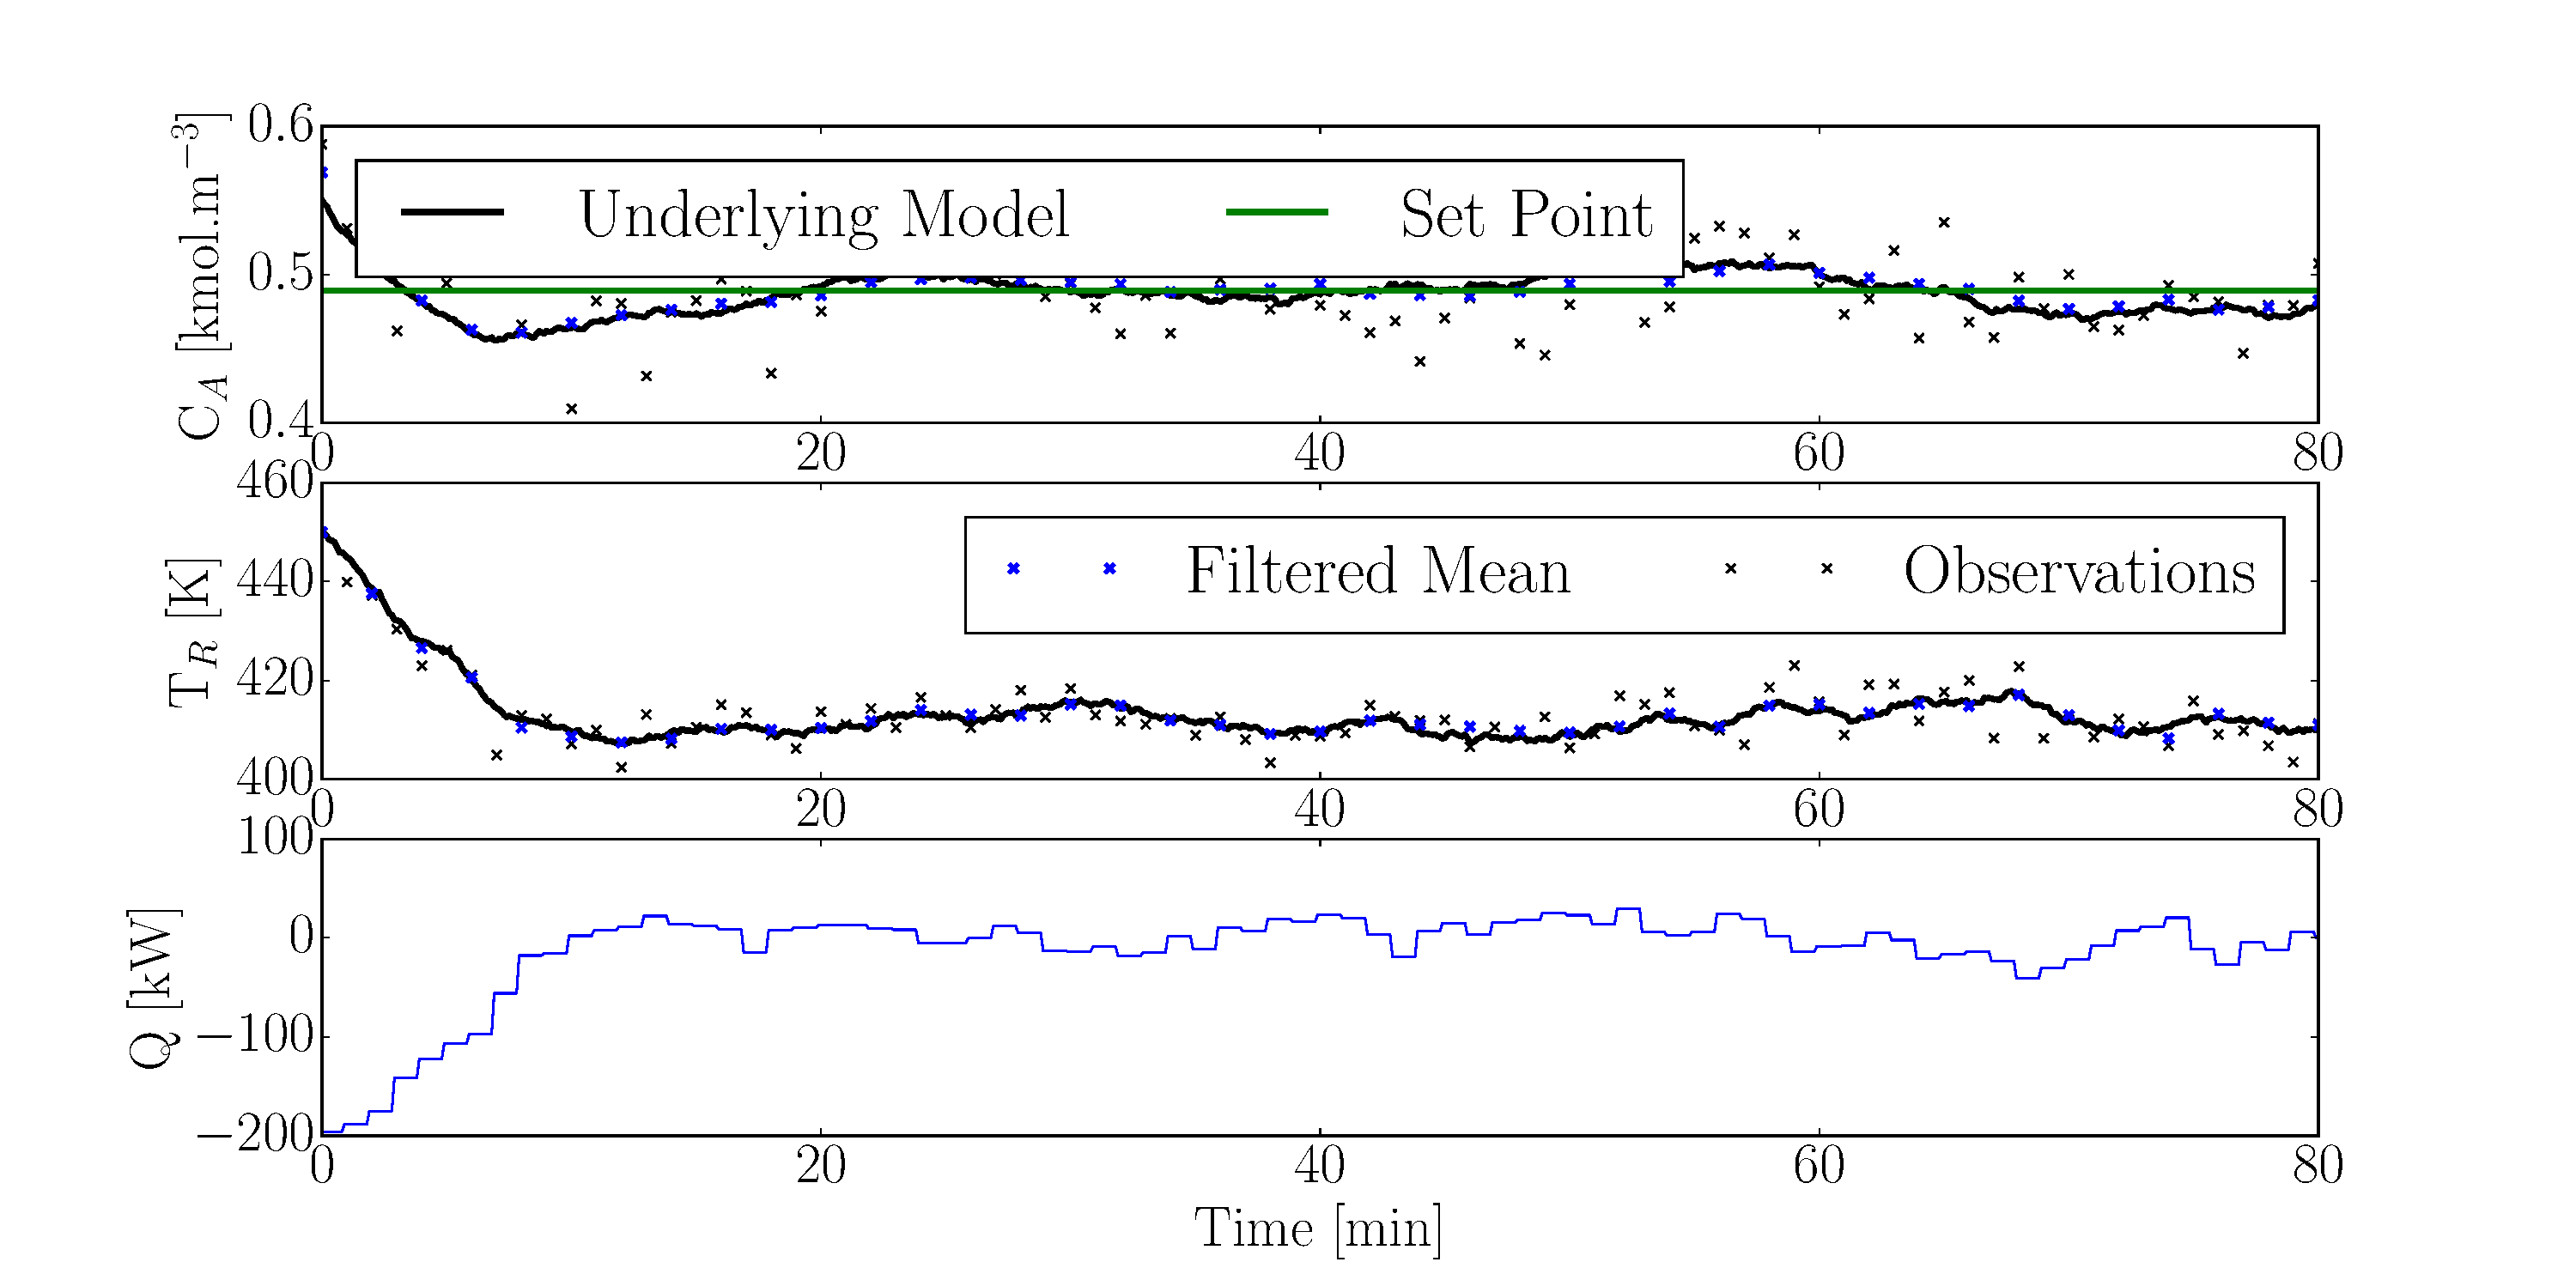
\includegraphics[scale=0.25]{lin_mod_lqg.pdf}
\caption{Unconstrained LQG regulator tracking with initial condition $(0.55, 450)$ and measuring both states.}
\label{fig_lin_mod_lqg}
\end{figure}
The average heat energy usage (controller input) over the simulation run is 214 kJ/min. The average set point error is 2.38\% over the same 40 min time period.
 
Next we illustrate the approach of using conventional deterministic MPC to control the stochastic system. The MPC formulation is shown in (\ref{eq_mpc_constrained_det1}). Using MPC allows us to easily add state and input constraints; this is a significant improvement over conventional LQG as discussed previously.
\begin{equation}
\begin{aligned}
&\underset{\mathbf{u}}{\text{min }} \frac{1}{2}\sum_{k=0}^{N-1} \left( \mu_k^TQ\mu_k + u_k^TRu_k \right) + \frac{1}{2}\mu_N^TP_f\mu_N \\
& \text{subject to } \mu_{t+1}=A\mu_t + Bu_t \\
&\text{and } \begin{pmatrix}
10 \\ 1
\end{pmatrix}^T \mu_t + 411 \geq 0 ~\forall ~t=1,...,N\\
& \text{and } |u_t| \leq 10000 ~\forall ~t=0,...,N-1\\
\end{aligned}
\label{eq_mpc_constrained_det1}
\end{equation}
We only use a single state constraint in this dissertation but the extension to multiple constraints is straightforward. The prediction and control horizon are equal to each other and set at 150 time steps i.e. 15 minutes into the future. We additionally constrain the magnitude of the inputs.

Since we have assumed normality the deterministic state inequality constraint can also be seen as an affine expected value constraint as shown in Theorem \ref{thrm_affine_expected_const}.

In Figure \ref{fig_lin_mod_kf_mean_track} we see the reference tracking and controller input for the deterministic MPC. The average heat energy input and set point error over the simulation run is 2.70\% and 222 kJ/min. Interestingly the average error is not much different but the controller requires more energy to track the setpoint without violating the constraints. This is reasonable because the additional constraints make problem (\ref{eq_mpc_constrained_det1}) a harder problem than (\ref{eq_lqg_linmod}).
\begin{figure}[H] 
\centering
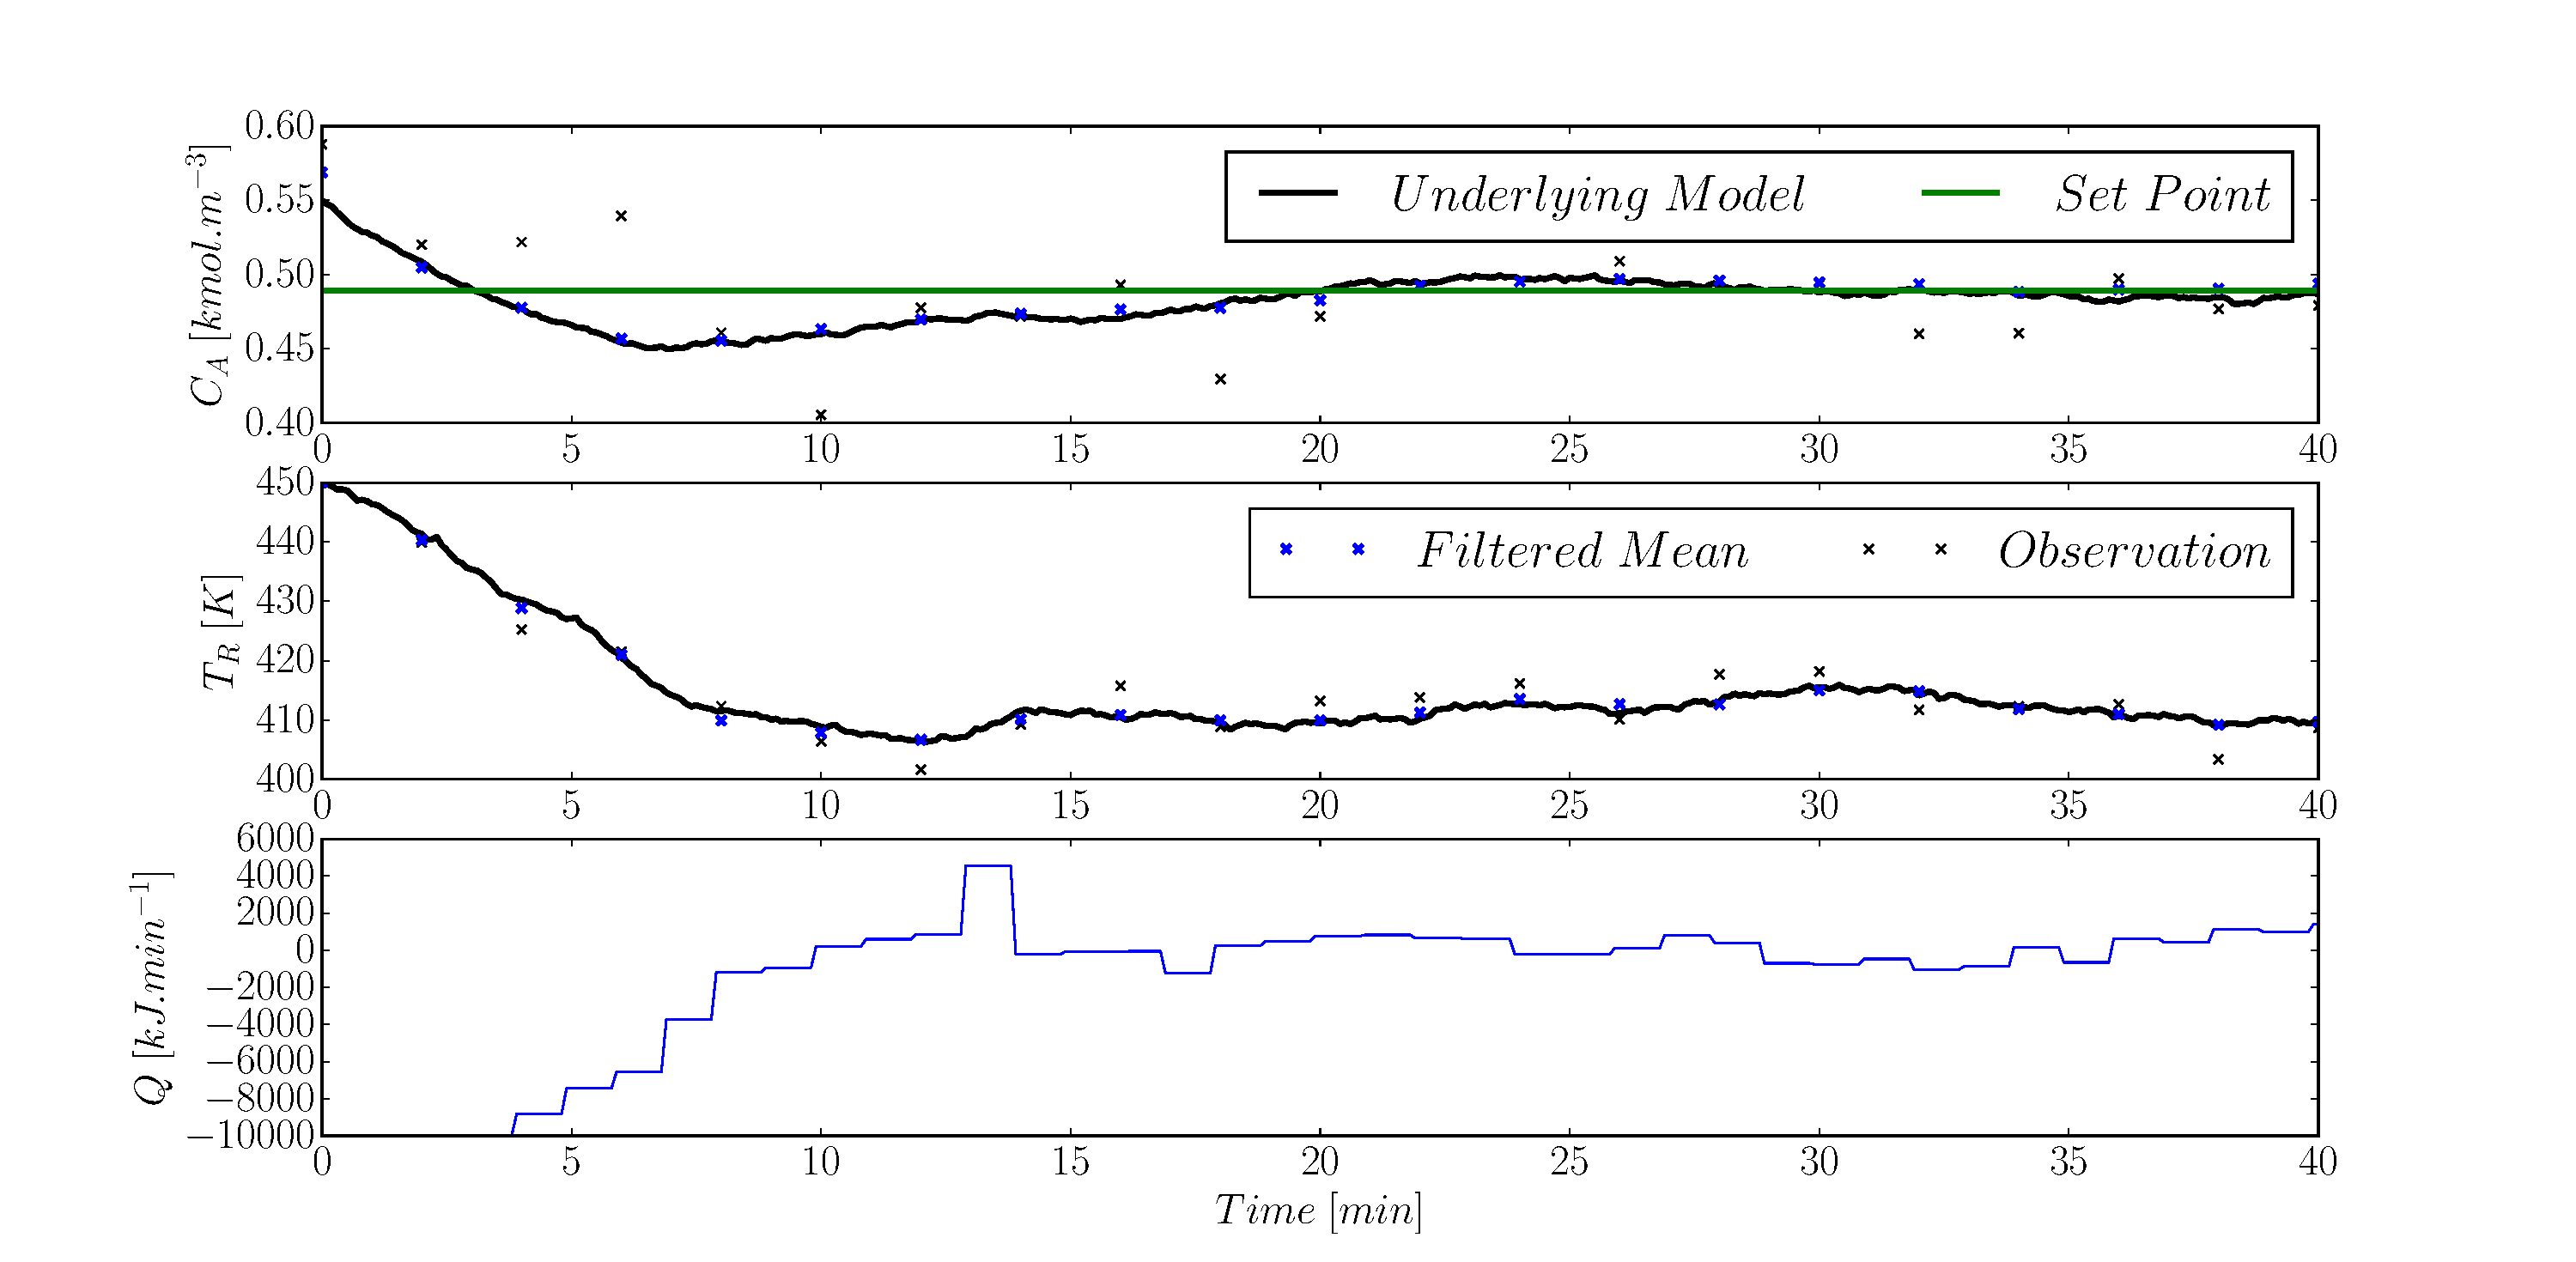
\includegraphics[scale=0.25]{lin_mod_kf_mean_track.pdf}
\caption{Deterministic constrained MPC tracking with initial condition $(0.55, 450)$ and measuring both states.}
\label{fig_lin_mod_kf_mean_track}
\end{figure}
Like the LQG controller, it is clear that we have noisy convergence to the set point. As mentioned previously we will never be able to achieve zero set point offset because of the noise term in the system dynamics (\ref{eq_lin_system}). Note that we have constrained the maximum magnitude of the inputs such that $|u_t| \leq 10000$ kJ/min. In the unconstrained case the controller required a maximum absolute input magnitude of over $12000$ kJ/min; the ability to naturally constrain the input can be practically very useful. The benefit of MPC is apparent here.

In Figure \ref{fig_lin_mod_kf_mean_ss} we see the corresponding state space trajectory of the system together with the state constraint.
\begin{figure}[H] 
\centering
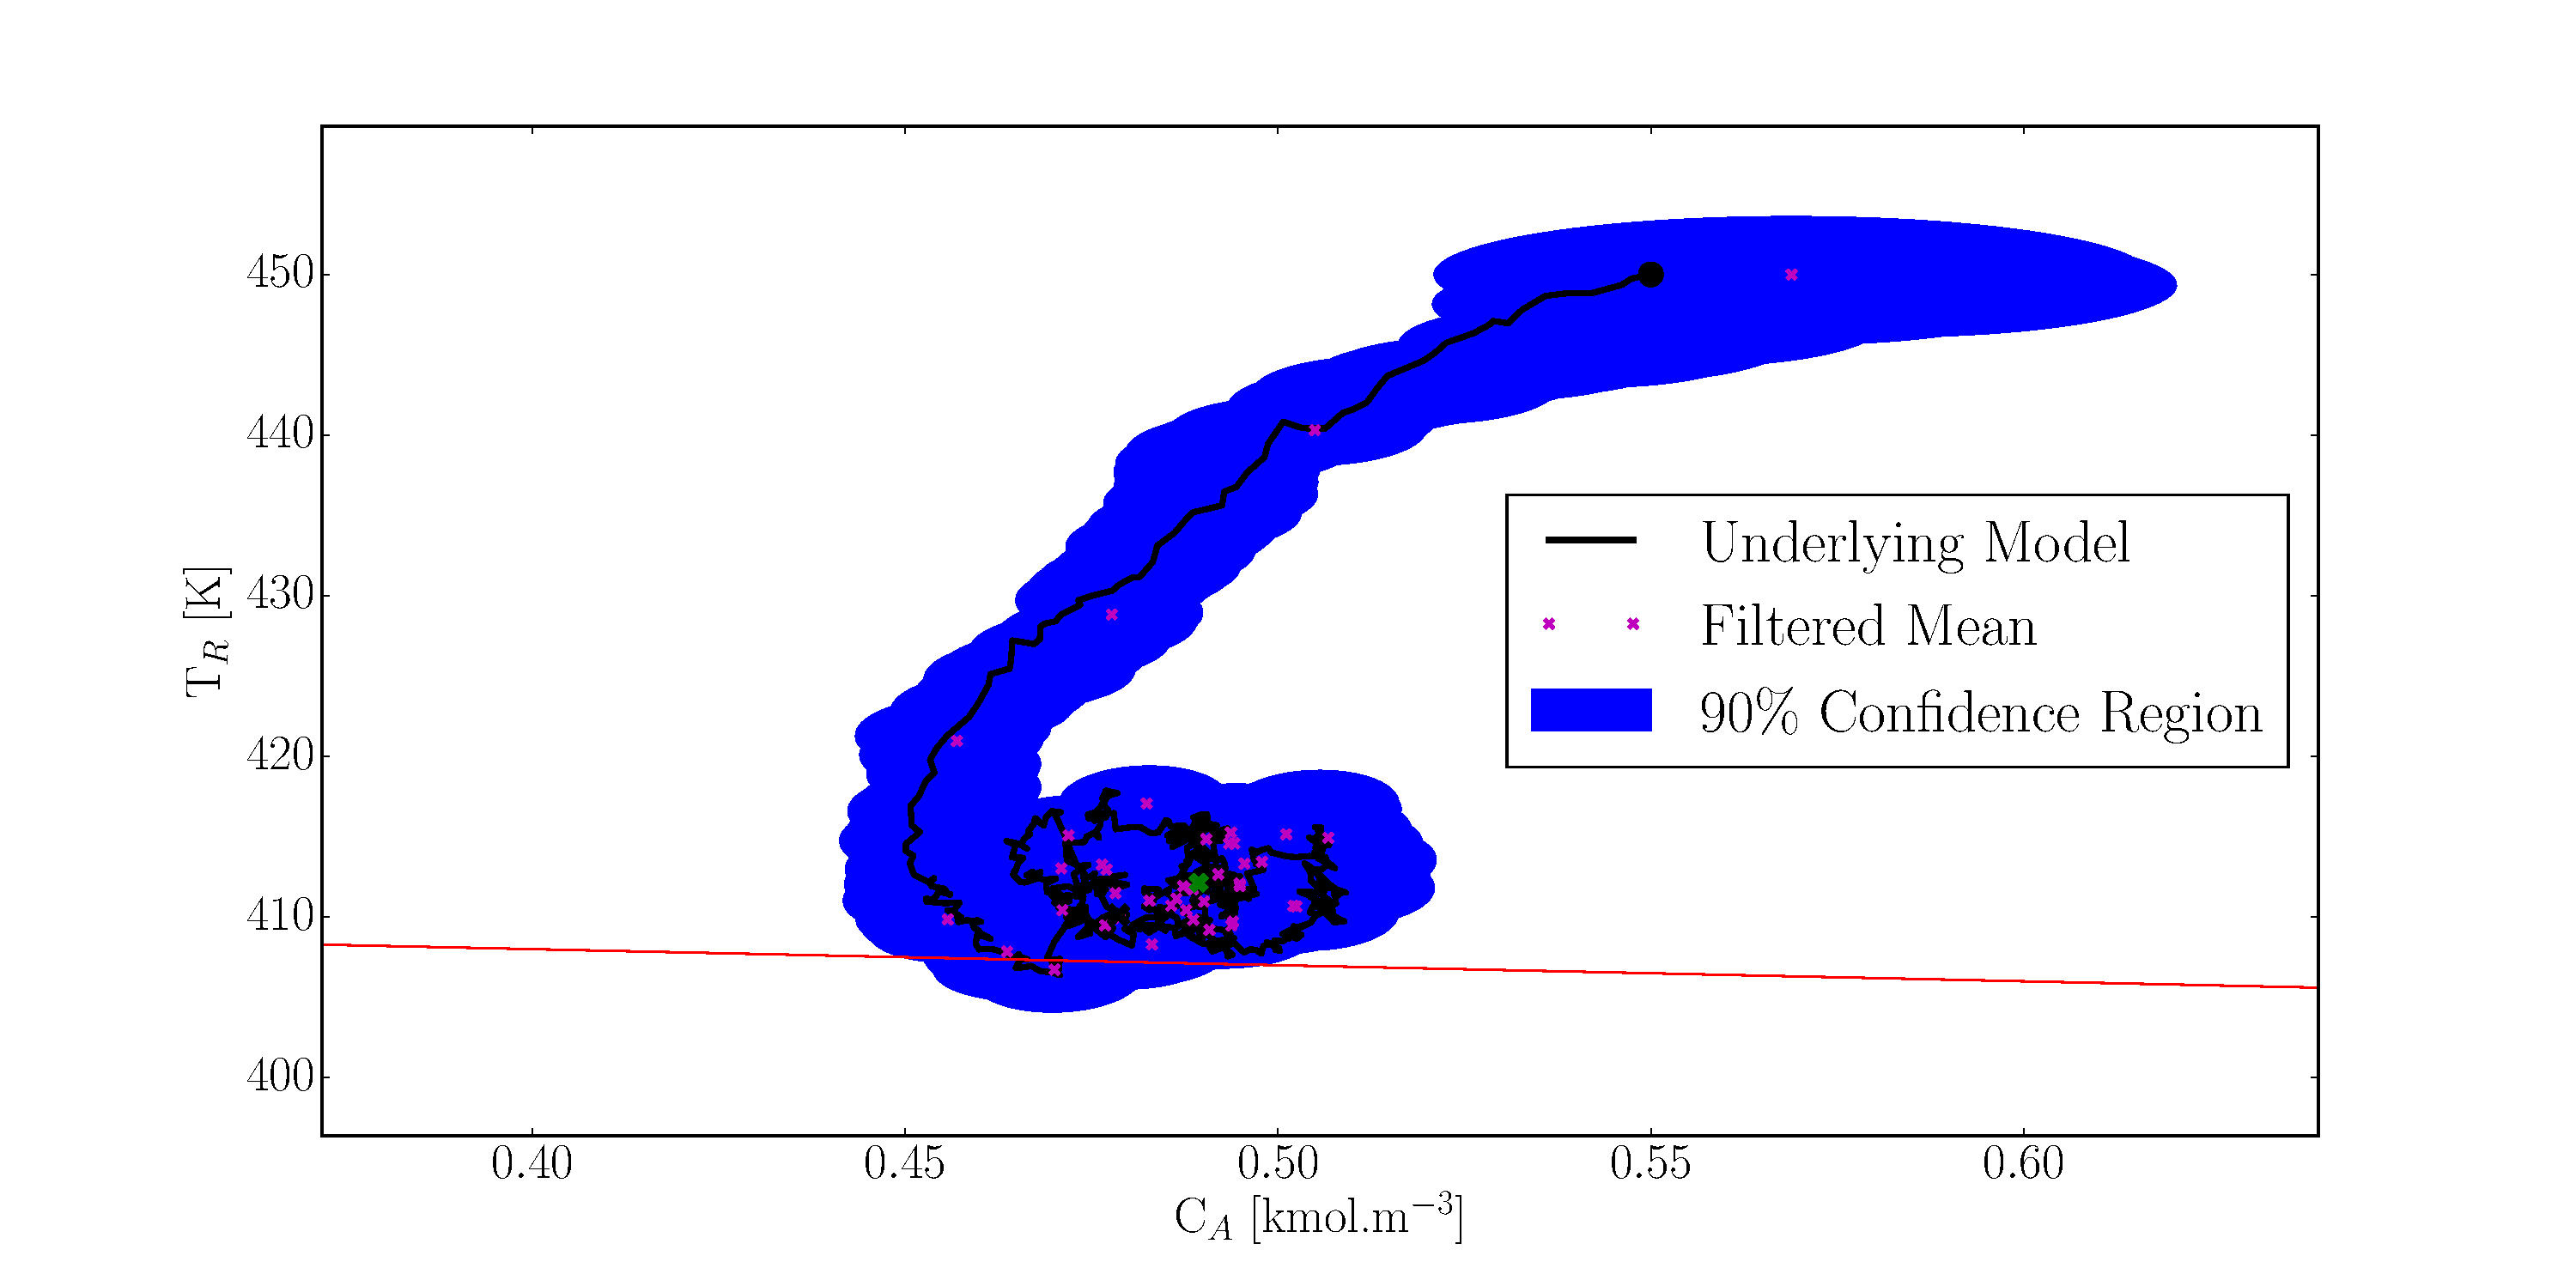
\includegraphics[scale=0.25]{lin_mod_kf_mean_ss.pdf}
\caption{Deterministic MPC state space trajectory with initial condition $(0.55, 450)$ and measuring both states.}
\label{fig_lin_mod_kf_mean_ss}
\end{figure}
While the predicted mean state estimates do not violate the constraint (due to the optimisation constraints) the actual underlying system does.  This is clearly seen if one inspects the confidence region around the lower state estimates. The confidence region is deeply violated by the constraint which implies that it is likely that the underlying system might. This is clearly a problem from a control point of view; the deterministic MPC cannot ensure that the constraint is satisfied.

We remedy this situation by introducing the stochastic MPC as discussed in Theorem \ref{thrm_mpc_stoch_to_det} and shown in (\ref{eq_mpc_linmod_kf_cons}) for convenience. Note that $d^T = (10, 1)$ and $e=411$ as before. By consulting a Chi-Squared Distribution table we set $k^2 = 4.6052$ which corresponds to the chance constraint $\text{Pr}(d^Tx_t + e \geq 0) \geq 90\% ~\forall ~t=1,...,N$.
\begin{equation}
\begin{aligned}
&\underset{\mathbf{u}}{\text{min }} \frac{1}{2}\sum_{k=0}^{N-1} \left( \mu_k^TQ\mu_k + u_k^TRu_k \right) + \frac{1}{2}\mu_N^TP_f\mu_N + \frac{1}{2}\sum_{k=0}^N \text{tr}(Q\Sigma_k) \\
& \text{subject to } \mu_{t+1}=A\mu_t + Bu_t \\
& \text{and } \Sigma_{t+1} = W+A\Sigma_t A^T \\
& \text{and } d^T\mu_t + e \geq k\sqrt{d^T \Sigma_t d} ~\forall ~t=1,...,N\\
& \text{and } |u_t| \leq 10000 ~\forall ~t=0,...,N-1\\
\end{aligned}
\label{eq_mpc_linmod_kf_cons}
\end{equation}
Note that problem (\ref{eq_mpc_linmod_kf_cons}) is harder than (\ref{eq_mpc_constrained_det1}) due to the added constraint and thus we expect that the system will require greater controller input to satisfy the constraint. 

In Figure \ref{fig_lin_mod_kf_var90_track} we see that the stochastic MPC is able to track the set point in a similar manner as the LQG controller and deterministic MPC. The total average heat input and set point error over the simulation run is 290 kJ/min and 2.95\% respectively. This problem is harder than the preceding one due to the additional constraint and thus more energy is required. 
\begin{figure}[H] 
\centering
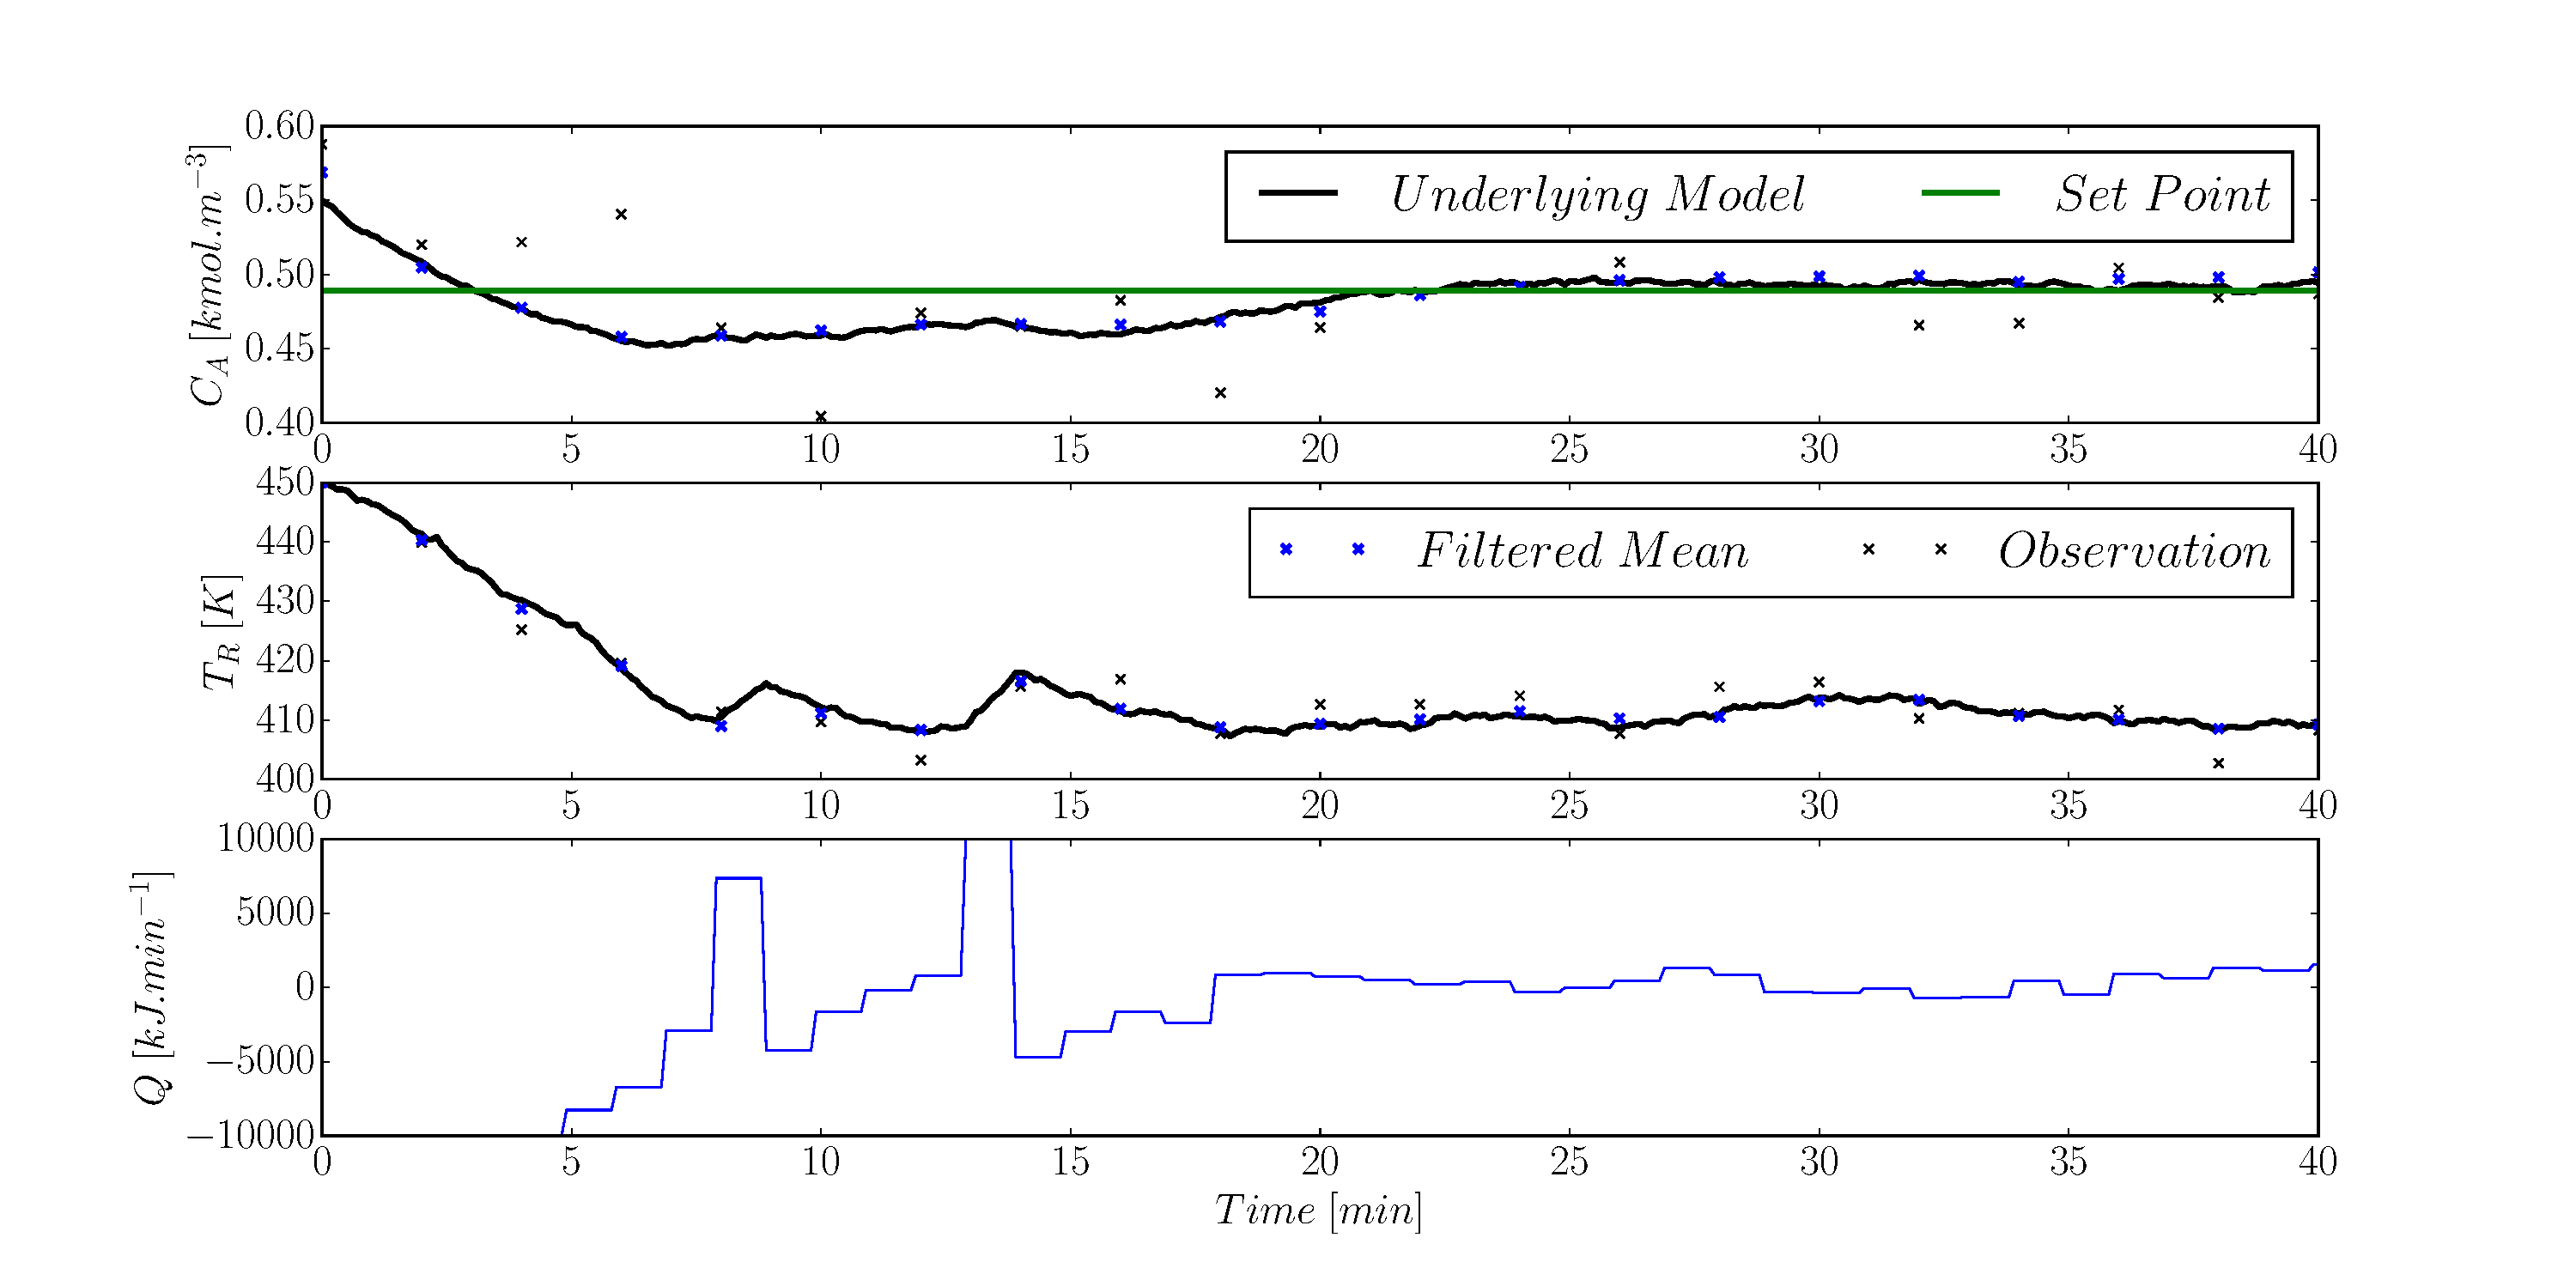
\includegraphics[scale=0.25]{lin_mod_kf_var90_track.pdf}
\caption{Stochastic constrained MPC tracking with initial condition $(0.55, 450)$ and measuring both states.}
\label{fig_lin_mod_kf_var90_track}
\end{figure}
However, the benefit of adding the stochastic constraint is apparent in Figure \ref{fig_lin_mod_kf_var90_ss}. It is clear that the constraint on the underlying state is not violated.
\begin{figure}[H] 
\centering
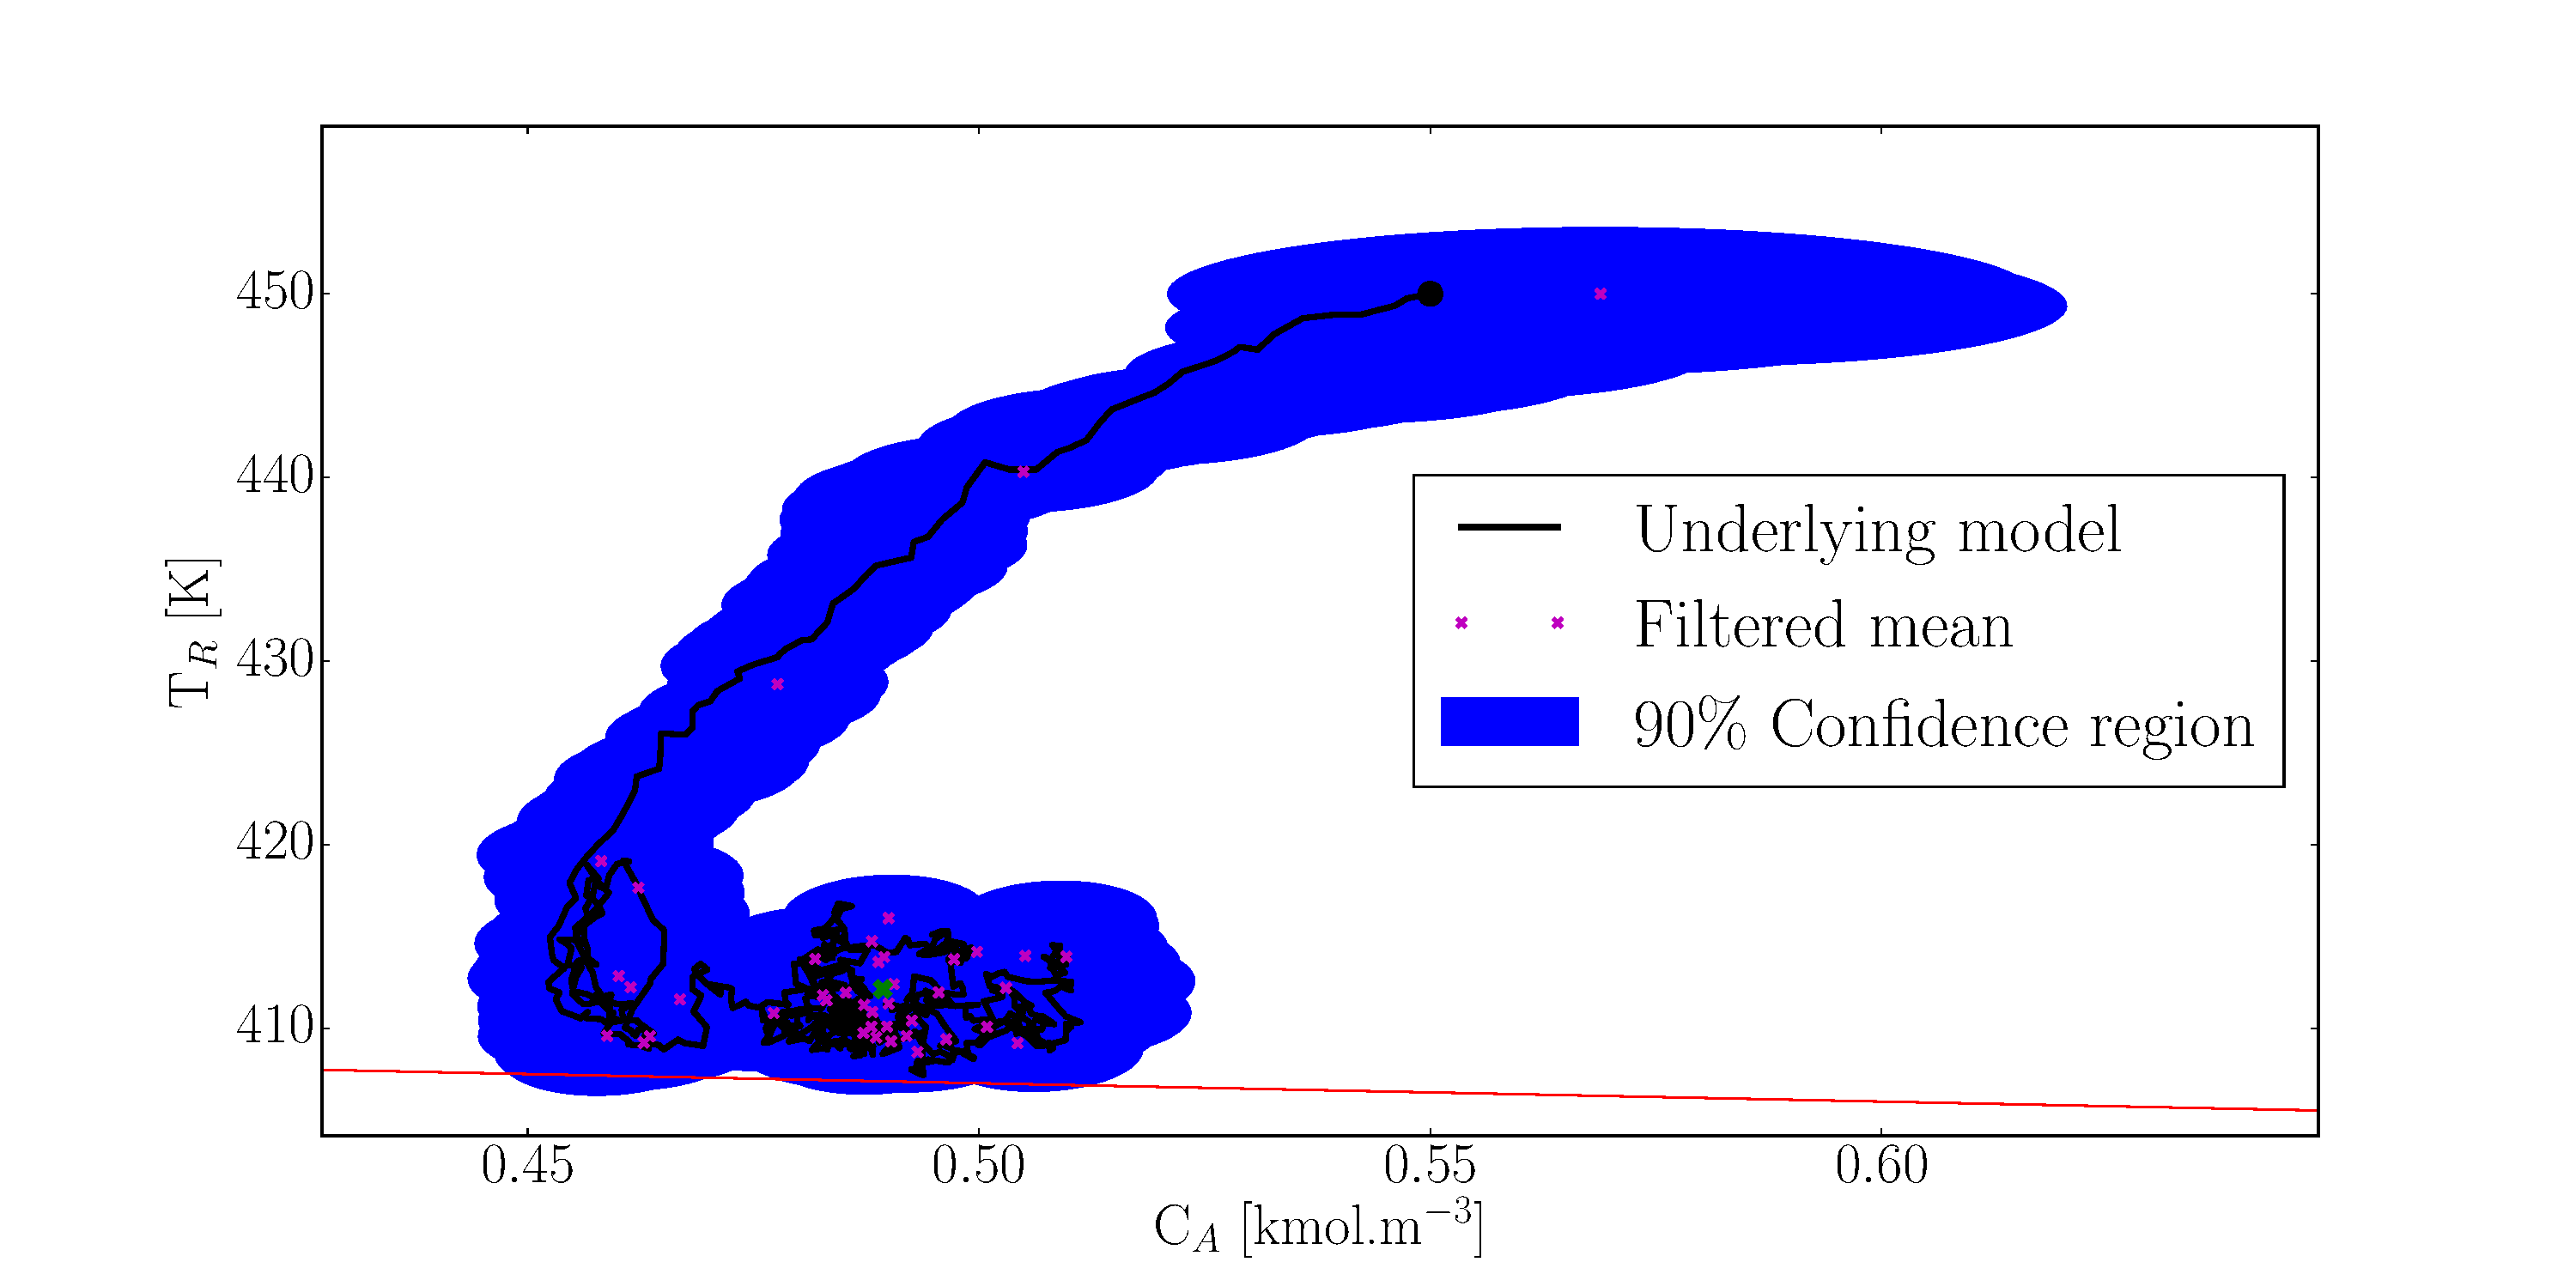
\includegraphics[scale=0.25]{lin_mod_kf_var90_ss.pdf}
\caption{Stochastic MPC state space trajectory with initial condition $(0.55, 450)$ and measuring both states.}
\label{fig_lin_mod_kf_var90_ss}
\end{figure}
Since the stochastic constraint is only enforced with probability 90\% it is possible that the underlying system can come ``close" to the constraint. This then has the consequence that the posterior confidence region marginally violates (spills over) the constraint as seen in the lower regions of Figure \ref{fig_lin_mod_kf_var90_ss}.

It is interesting to investigate what effect increasing the probability that the chance constraint is satisfied will have on the system. To this end we modify the chance constraint of (\ref{eq_mpc_linmod_kf_cons}) such that $k^2 = 13.8155$ which corresponds to the chance constraint $\text{Pr}(d^Tx_t + e \geq 0) \geq 99.9\% ~\forall ~t=1,...,N$. We expect that the underlying system will be moved further away from constraint due to this added level of conservativeness.

In Figure \ref{fig_lin_mod_kf_var999_track} we see that the stochastic MPC still tracks the set point and Figure \ref{fig_lin_mod_kf_var999_ss} shows that the expected behaviour is realised. 
\begin{figure}[H] 
\centering
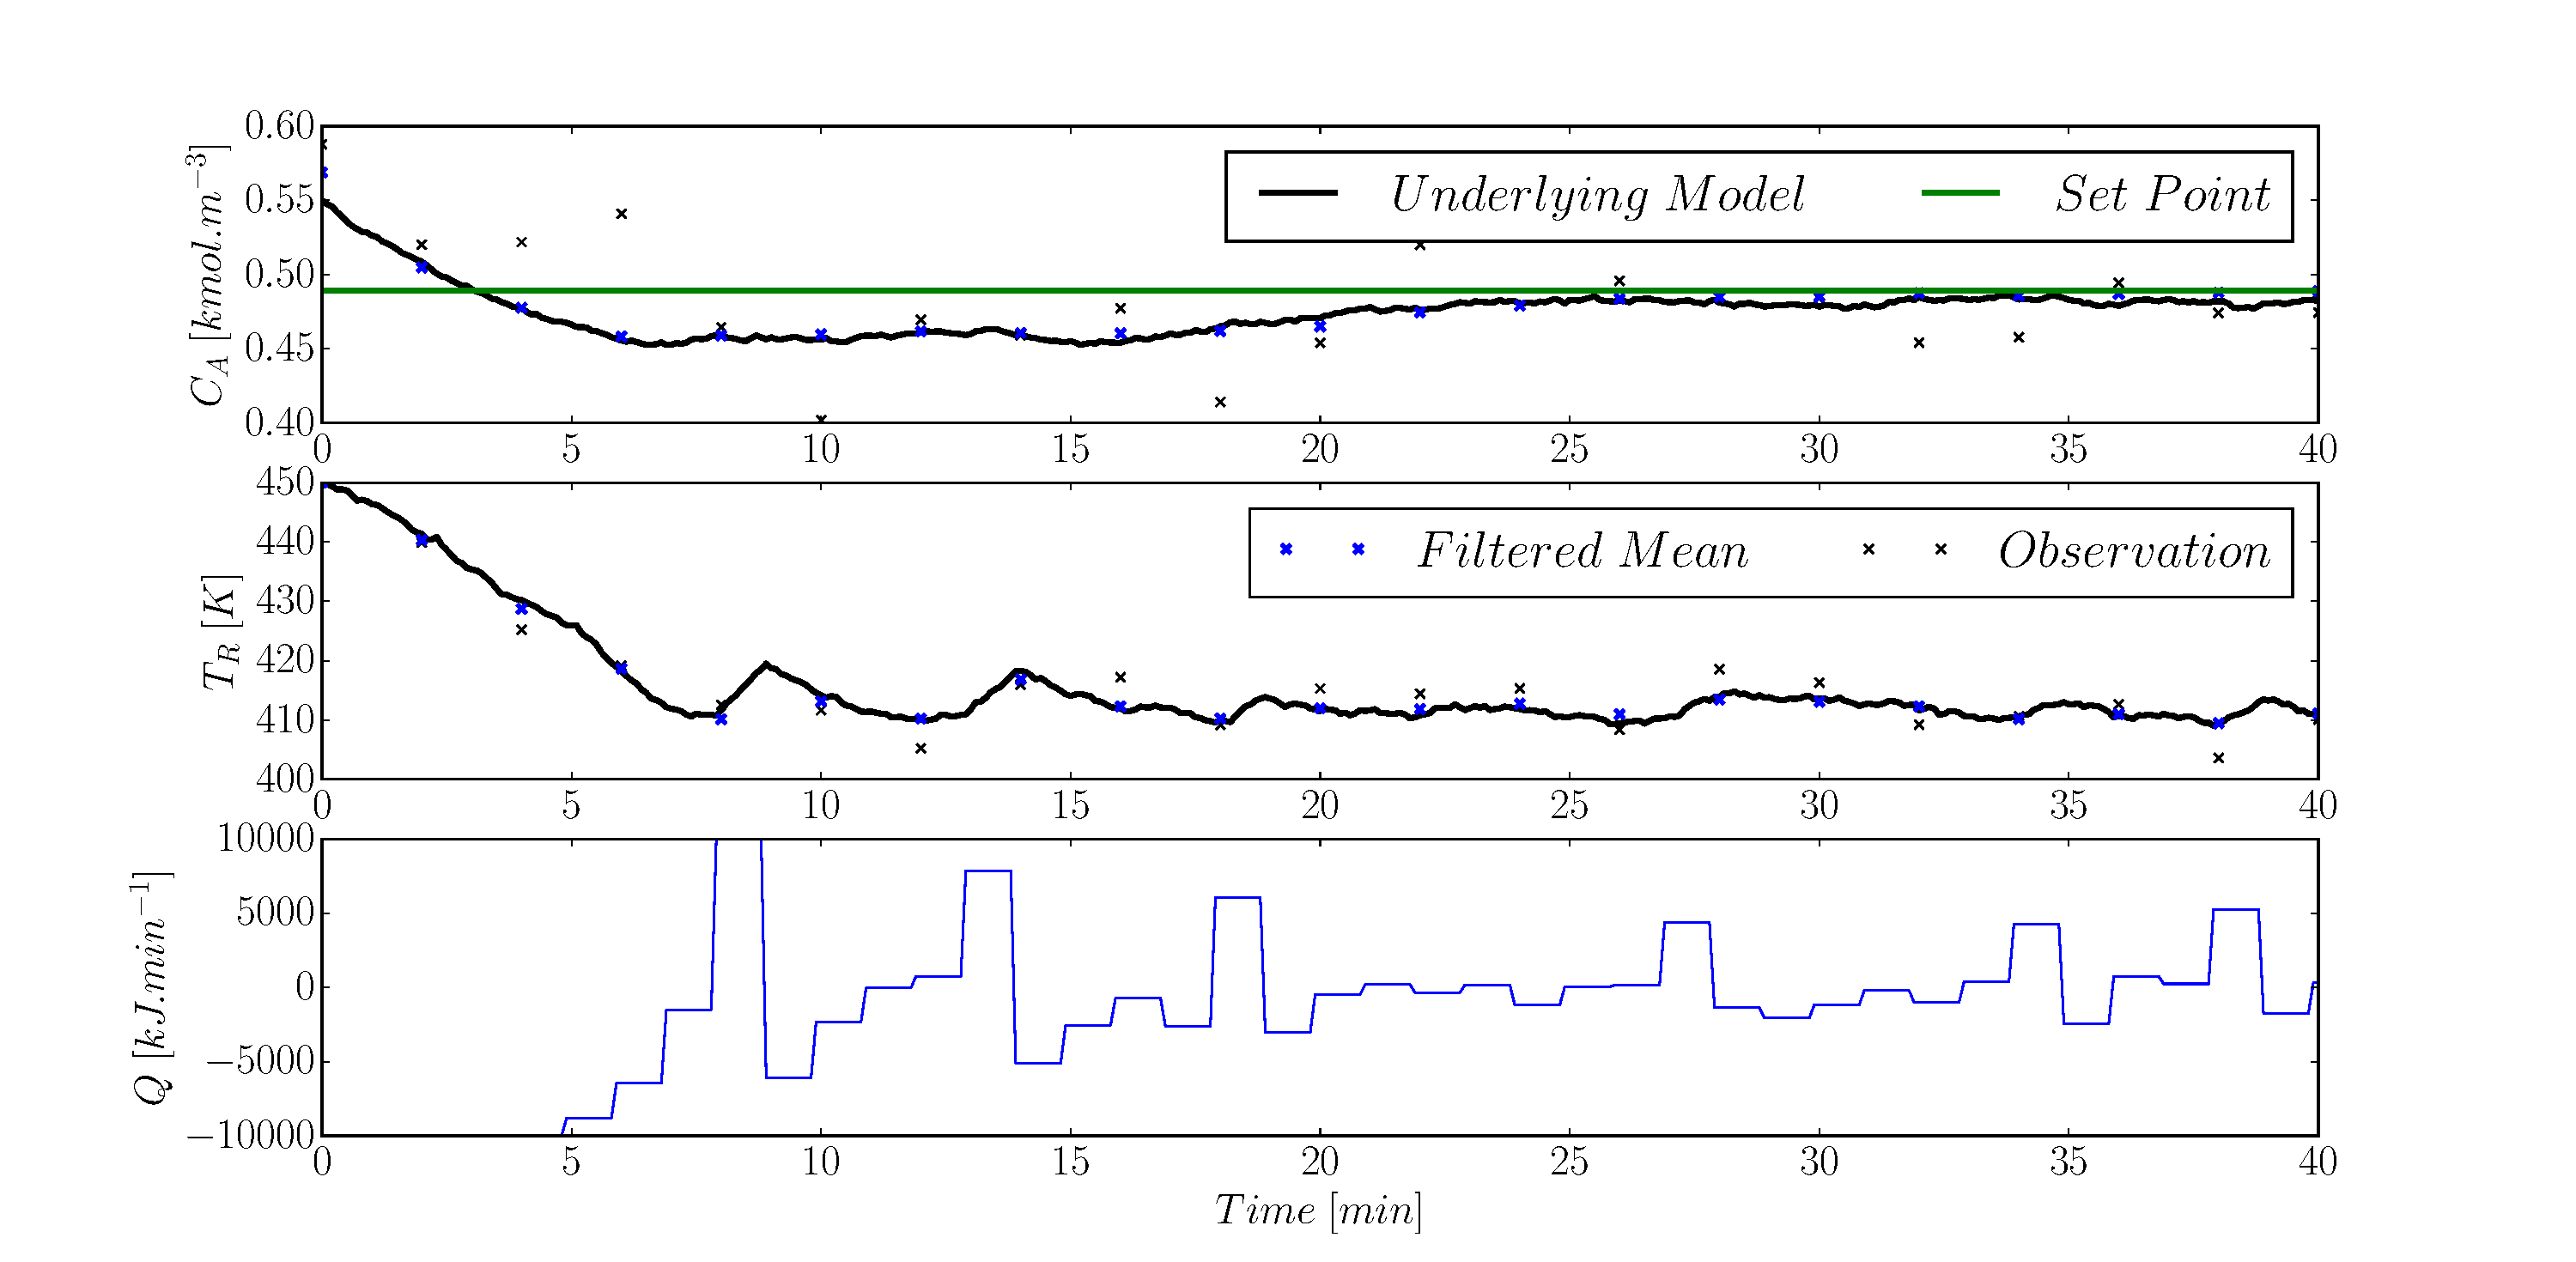
\includegraphics[scale=0.25]{lin_mod_kf_var999_track.pdf}
\caption{Stochastic constrained MPC tracking with initial condition $(0.55, 450)$ and measuring both states. The chance constraint is set at 90\%.}
\label{fig_lin_mod_kf_var999_track}
\end{figure}
The average heat input and average set point error is 3.73\% and 351 kJ/min. The added conservativeness of the MPC prevents it from attempting to get to the set point as fast as the previous stochastic MPC; this causes the higher average error but the constraints are satisfied more robustly. As before, the control problem is harder and thus requires more energy.

In Figure \ref{fig_lin_mod_kf_var999_ss} we see the 90\% confidence region is above the constraint. Since the probability that the predicted states are close to the constraint is much lower than before we see that the confidence region satisfies the constraint everywhere.
\begin{figure}[H] 
\centering
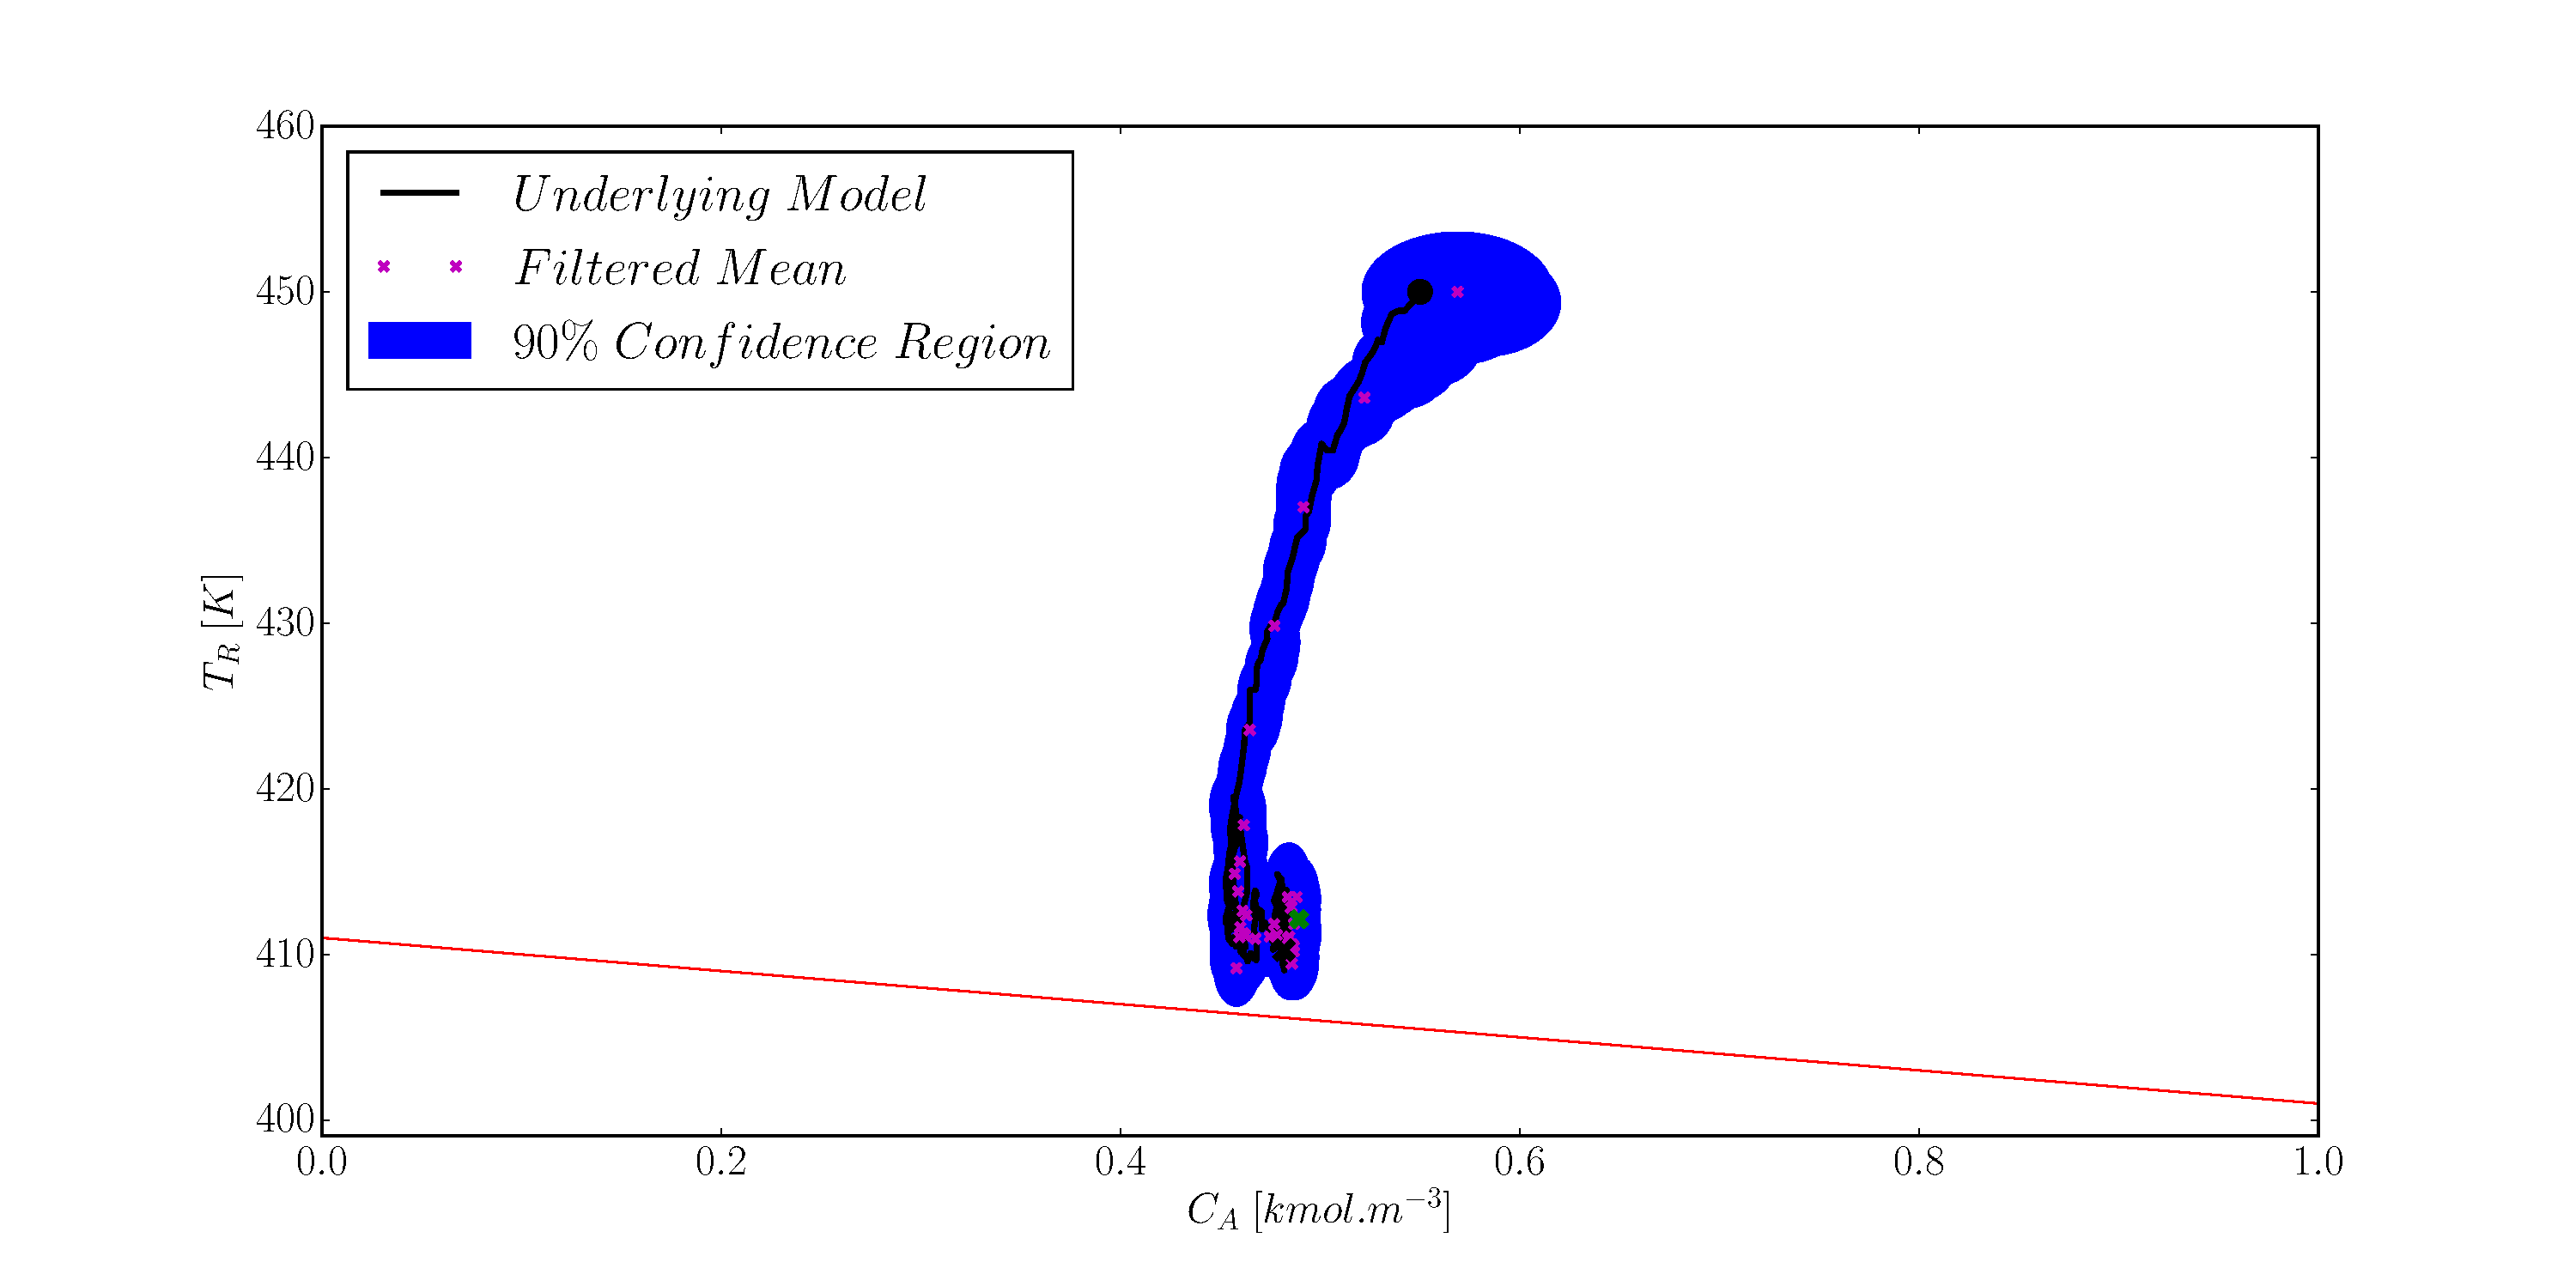
\includegraphics[scale=0.25]{lin_mod_kf_var999_ss.pdf}
\caption{Stochastic MPC state space trajectory with initial condition $(0.55, 450)$ and measuring both states. The chance constraint is set at 99.9\%.}
\label{fig_lin_mod_kf_var999_ss}
\end{figure}
It would also be correct to infer that $k$ can be used as an empirical measure of the inherent stochastic conservativeness of the resulting controller. That is, lower values of $k$ indicate a more aggressive controller which may violate the chance constraints and higher values of $k$ indicate a more conservative controller. This can be useful for systems where the normal assumption is not valid but one would still like to enforce stochastic constraints in some empirical sense. 

We have made the strong assumption that the system dynamics remain linear and Gaussian even under the MPC control law which is not necessarily linear \cite{mac}. Clearly if the system is far from Gaussian the Gaussian approach to simplifying the chance constraint will not be valid. Fortunately this is relatively simple to check and serves as a good way of measuring controller health. That is, the more Gaussian the filtered distributions are, the better the linear stochastic controller will work. 

Kullback-Leibler Divergence was introduced in Theorem \ref{thrm_kl_sample} to estimate the degree to which samples match a given distribution. From Section \ref{sec_inf_nonlin_mods} we know that given enough particles a Particle Filter can accurately represent any distribution. Thus we temporarily replace the Kalman Filter with a Particle filter and use Theorem \ref{thrm_kl_sample} to estimate the degree of normality of the posterior state distributions.

Figure \ref{fig_lin_mod_kl} shows the degree to which the underlying distribution is Gaussian. Since we cannot use an infinite amount of particles we compare the sampled Gaussian distribution approximation to a baseline.   
\begin{figure}[H] 
\centering
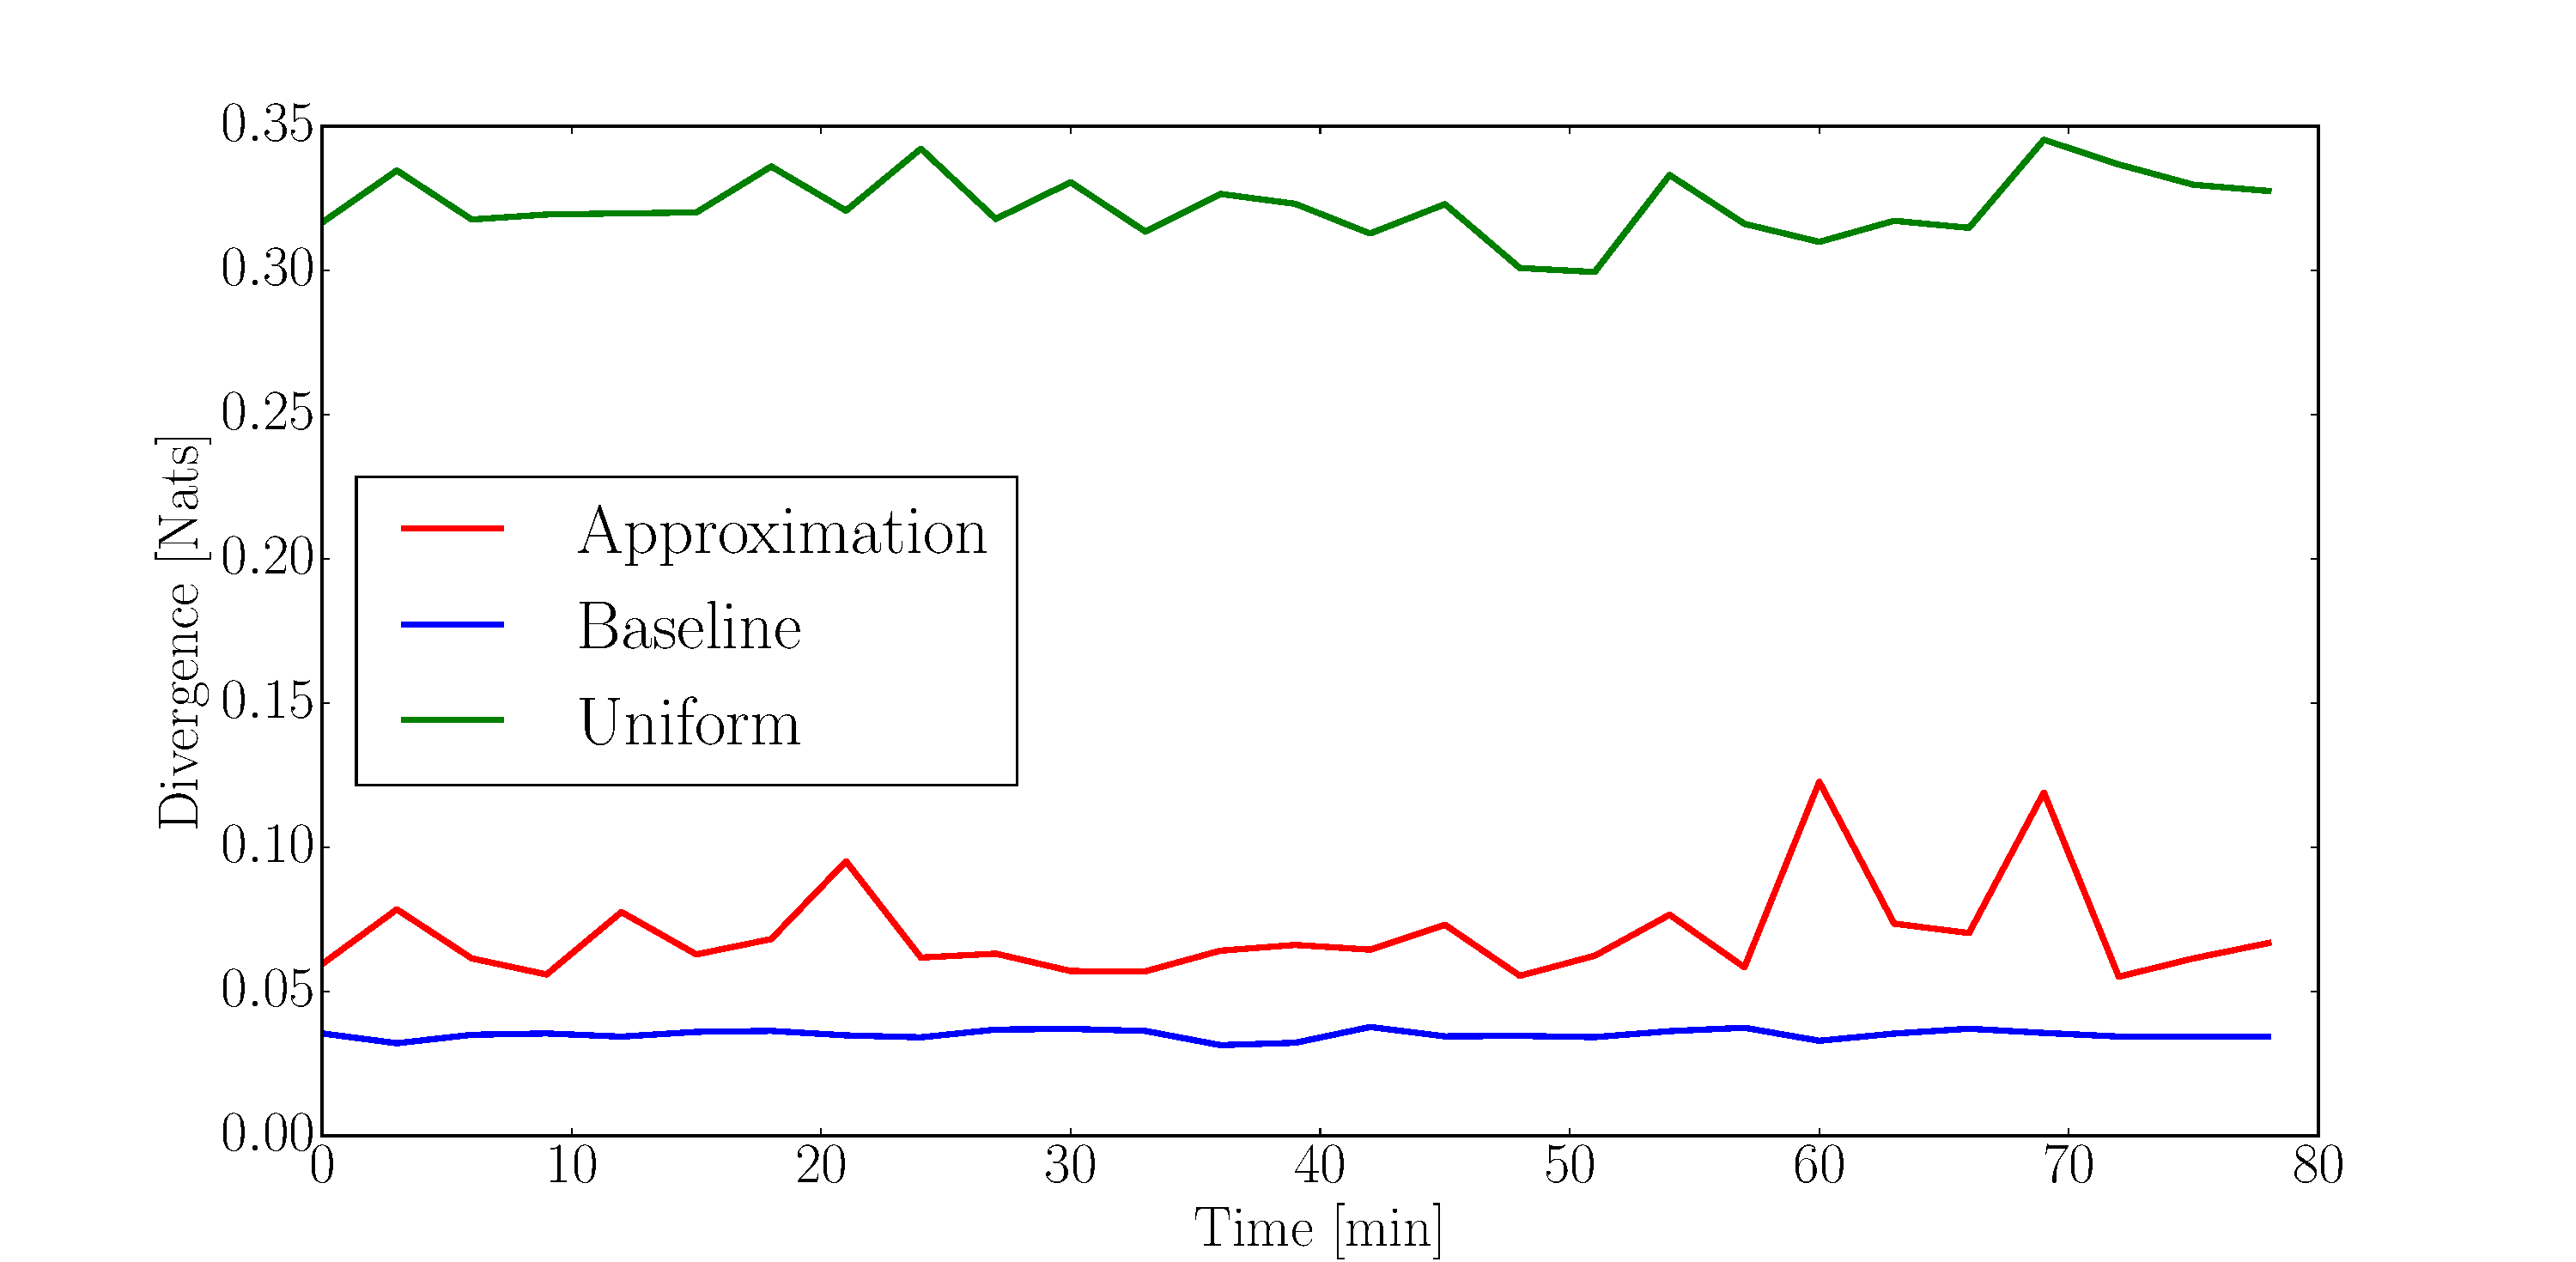
\includegraphics[scale=0.25]{lin_mod_kl.pdf}
\caption{Kullback-Leibler Divergence between the assumed Gaussian distribution and actual distribution using 5000 particles.}
\label{fig_lin_mod_kl}
\end{figure}
The approximation curve in Figure \ref{fig_lin_mod_kl} shows how much the samples diverge from the Gaussian distribution approximated using the samples. The baseline curve shows how much the Gaussian distribution diverges from samples of the same distribution. One would expect the baseline curve to tend to zero as the number of particles tends to infinity. Sampling error causes divergence from zero for the baseline curve. Thus we can use the baseline curve as a crude measure of the  error introduced by sampling.

In Figure \ref{fig_lin_mod_kl} we see that the approximation is relatively close, within a factor of 2. This implies that even though we are using a non-linear control technique the posterior state distributions are still approximately Gaussian. 


\subsection{Nonlinear System}
In this section we consider the problem of controlling the full non-linear system with a linear model linearised around the unsteady operating point. The control goal is the same as before; the only difference between this section and Section \ref{sec_lin_sys_cont} is that the underlying plant is non-linear.

The linear control model and noise parameters are the same as (\ref{eq_linmod_params}). The control tuning parameters are the same as (\ref{eq_mpc_tuning}).

As before we first investigate the LQG controller. The control problem is the same as (\ref{eq_lqg_linmod}) but this time the underlying system is non-linear. Figure \ref{fig_nonlin_lqg} shows the unconstrained reference tracking results.
\begin{figure}[H] 
\centering
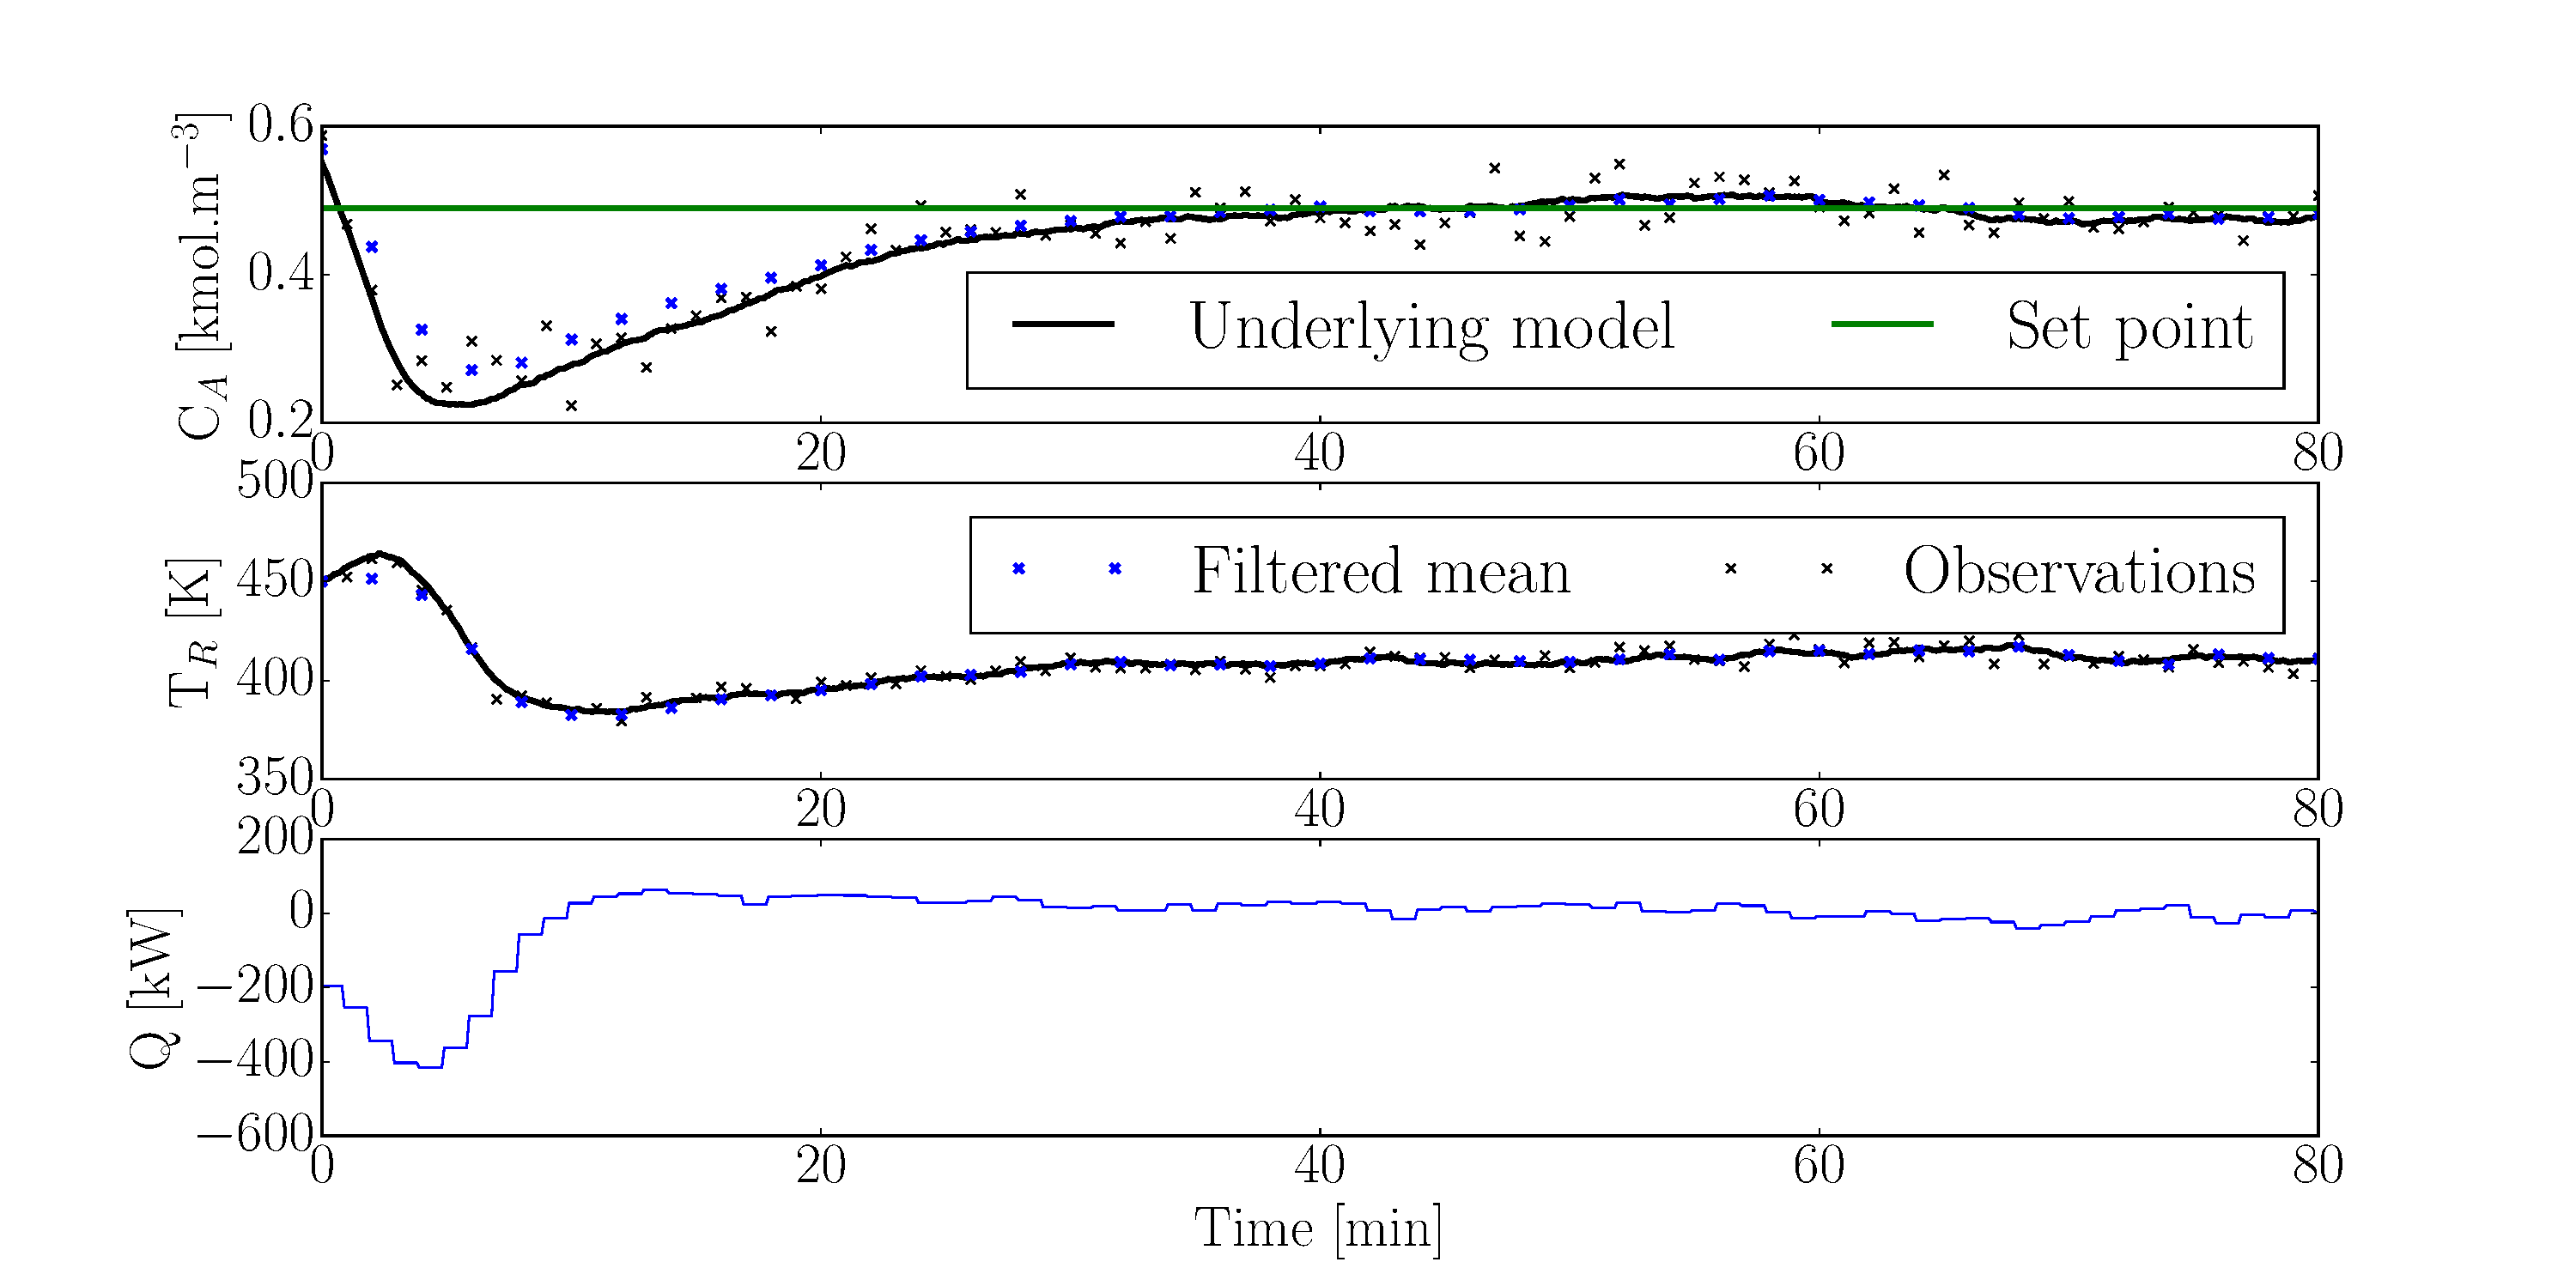
\includegraphics[scale=0.25]{nonlin_mod_lqg.pdf}
\caption{LQG regulator tracking with initial condition (0.55, 450) and measuring both states.}
\label{fig_nonlin_lqg}
\end{figure}
The average energy usage and concentration error was 302 kJ/min and 10.94\% respectively over the 80 min simulation time. Comparing Figures \ref{fig_lin_mod_lqg} and \ref{fig_nonlin_lqg} we see that the maximum absolute input energy is much greater with the non-linear underlying dynamics. This is not unexpected because the controller in both cases is linear: one expects that the plant-model mismatch to have a detrimental effect on control.

In the previous section we had a linear underlying model and linear control. Figure \ref{fig_lin_mod_kl} also demonstrated that the posterior state distributions were approximately Gaussian. Thus there was no reason to use non-linear inference algorithms like the Particle Filter introduced in Section \ref{sec_inf_nonlin_mods}. However, in this section we are using a non-linear underlying model and it might be advantageous to use a more sophisticated inference tool. We investigate using both a Kalman Filter and a Particle Filter for inference. In the setting of the Particle Filter we approximate the samples as Gaussian and use that for control.

As before we first investigate the deterministic MPC. The control problem is shown in (\ref{eq_mpc_constrained_det2}). Note that the constraints are different due to the expected extra difficulty introduced by the non-linear underlying model. 
\begin{equation}
\begin{aligned}
&\underset{\mathbf{u}}{\text{min }} \frac{1}{2}\sum_{k=0}^{N-1} \left( \mu_k^TQ\mu_k + u_k^TRu_k \right) + \frac{1}{2}\mu_N^TP_f\mu_N \\
& \text{subject to } \mu_{t+1}=A\mu_t + Bu_t \\
&\text{and } \begin{pmatrix}
10 \\ 1
\end{pmatrix}^T \mu_t + 400 \geq 0 ~\forall ~t=1,...,N\\
& \text{and } |u_t| \leq 20000 ~\forall ~t=0,...,N-1\\
\end{aligned}
\label{eq_mpc_constrained_det2}
\end{equation}
In Figure \ref{fig_nonlin_mod_kf_mean_track} we see that the deterministic MPC using the Kalman Filter for state inference does converge to the set point. The ability to naturally constrain the system is again highlighted in the input: as opposed to the -25 000 kJ/min required by the LQG controller the MPC manages to control the system while never requiring more than $|20000|$ kJ/min. 
\begin{figure}[H] 
\centering
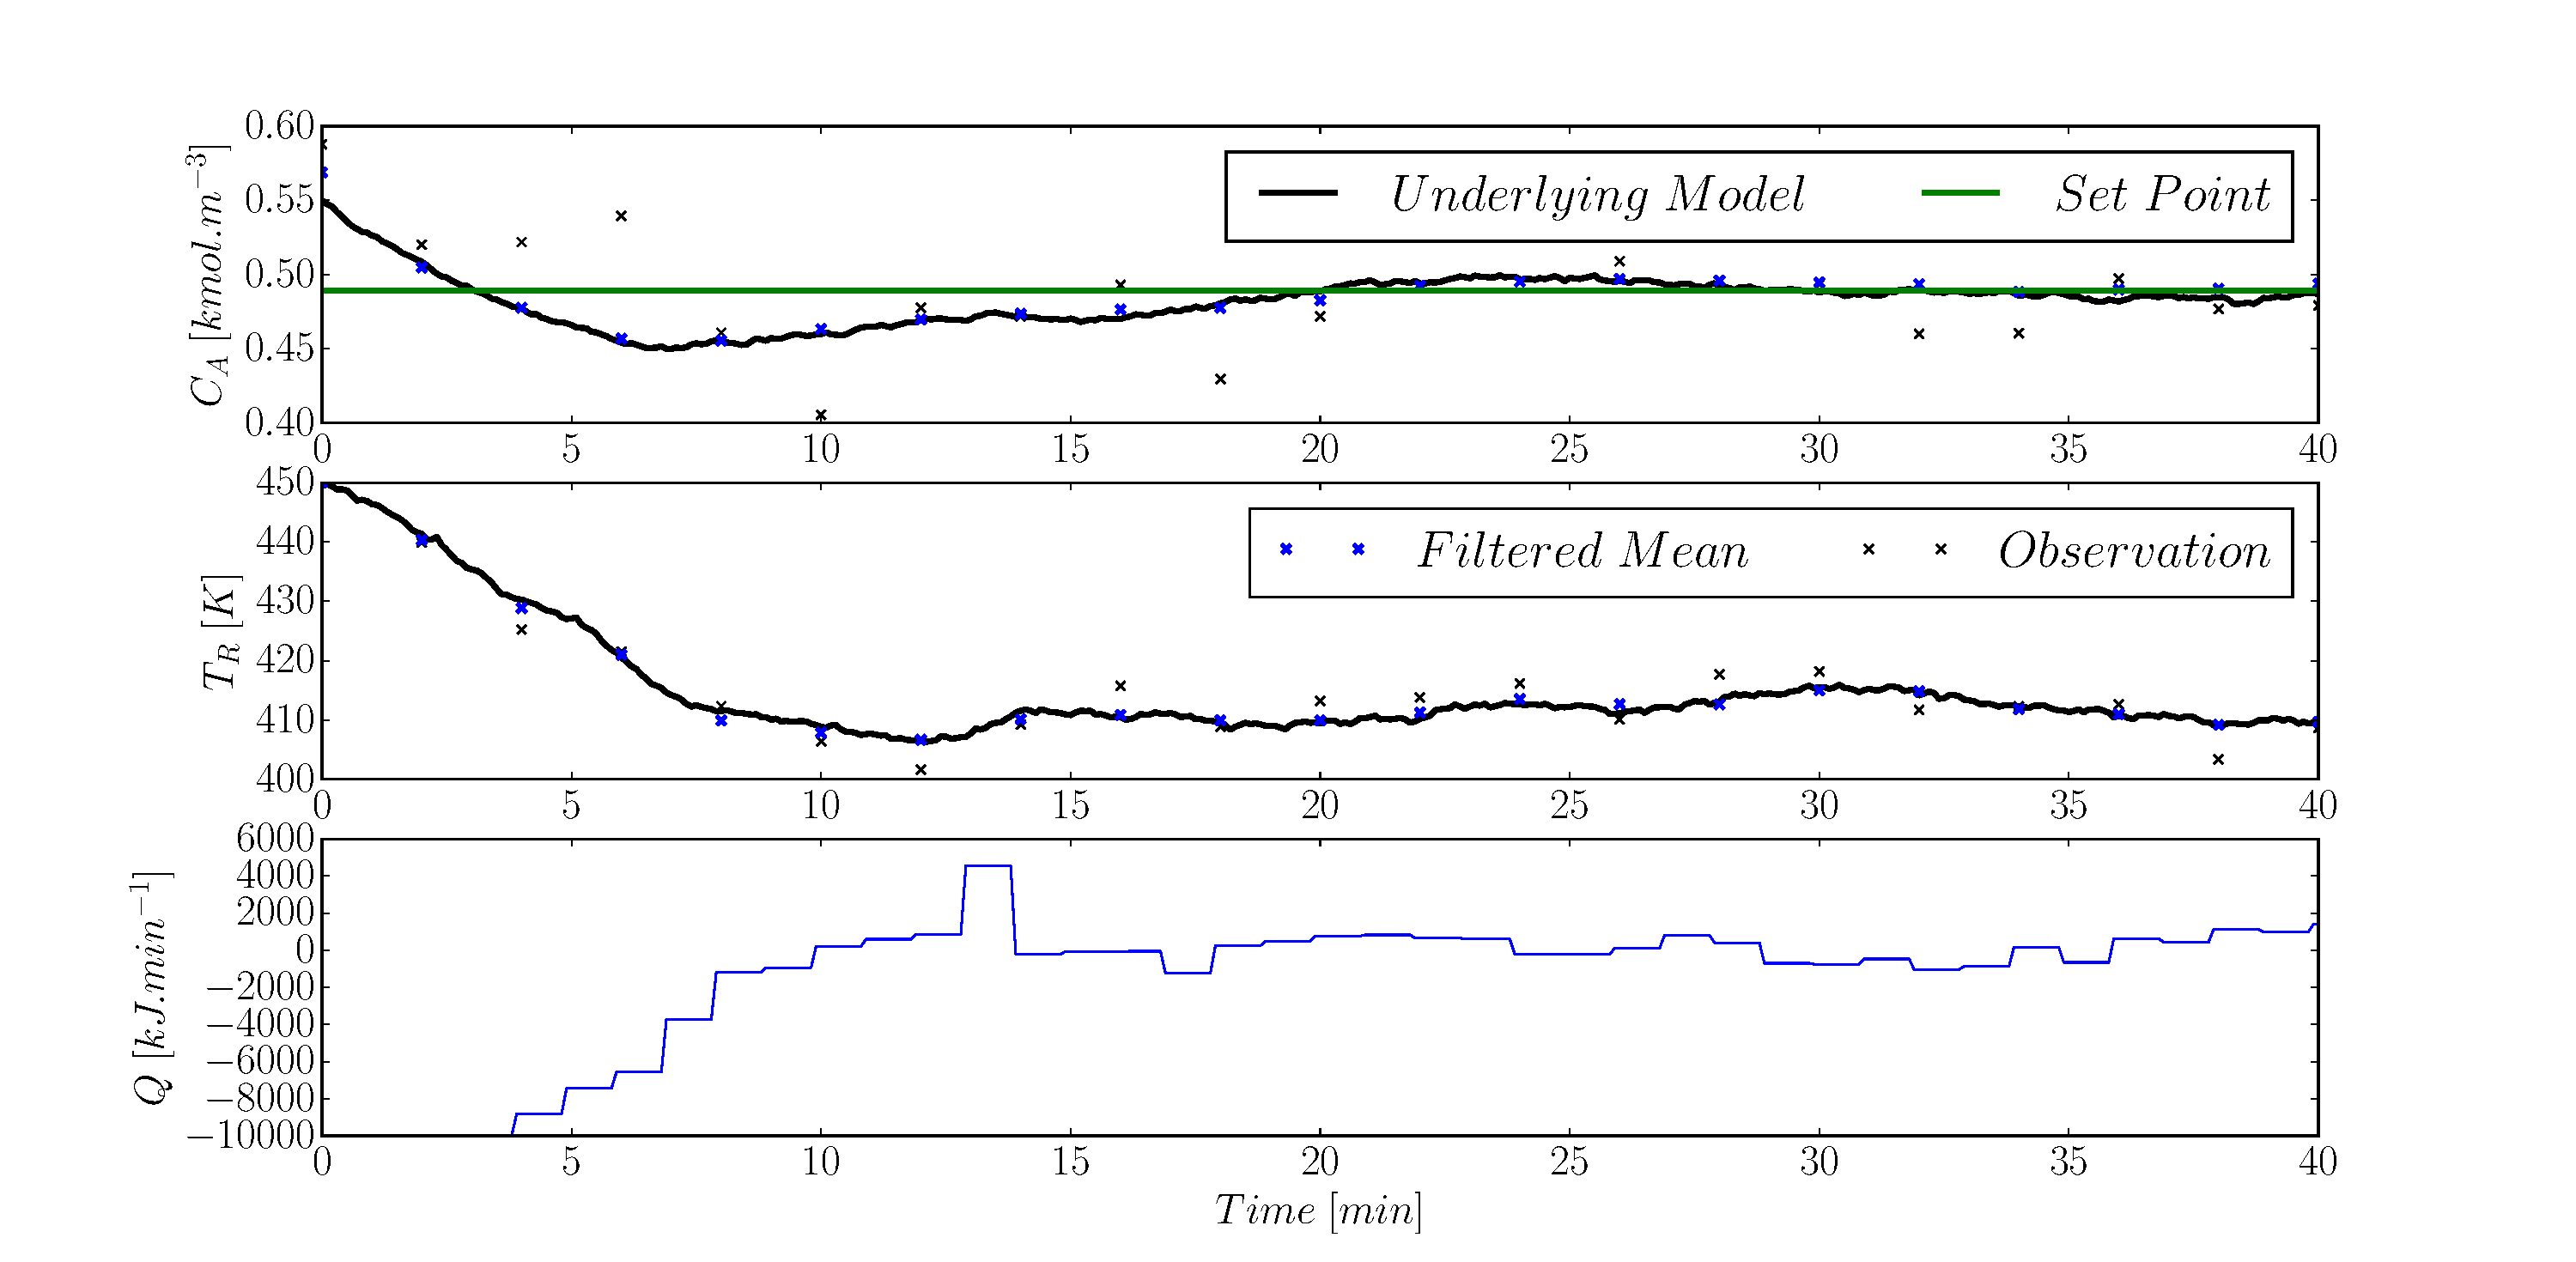
\includegraphics[scale=0.25]{lin_mod_kf_mean_track.pdf}
\caption{Deterministic constrained MPC reference tracking with initial condition $(0.55, 450)$ and measuring both states. The Kalman Filter is used for inference.}
\label{fig_nonlin_mod_kf_mean_track}
\end{figure} 
In Figure \ref{fig_nonlin_mod_kf_mean_ss} we see that the state constraint is violated just like Figure \ref{fig_lin_mod_kf_mean_ss}. We also see a somewhat unrealistic jagged state trajectory but this is just a numerical artefact. The average energy input and concentration error over the simulation run is 413 kJ/min and 14.53\% respectively. Once again the added constraints explain why the performance is degraded when compared to the LQG controller.
\begin{figure}[H] 
\centering
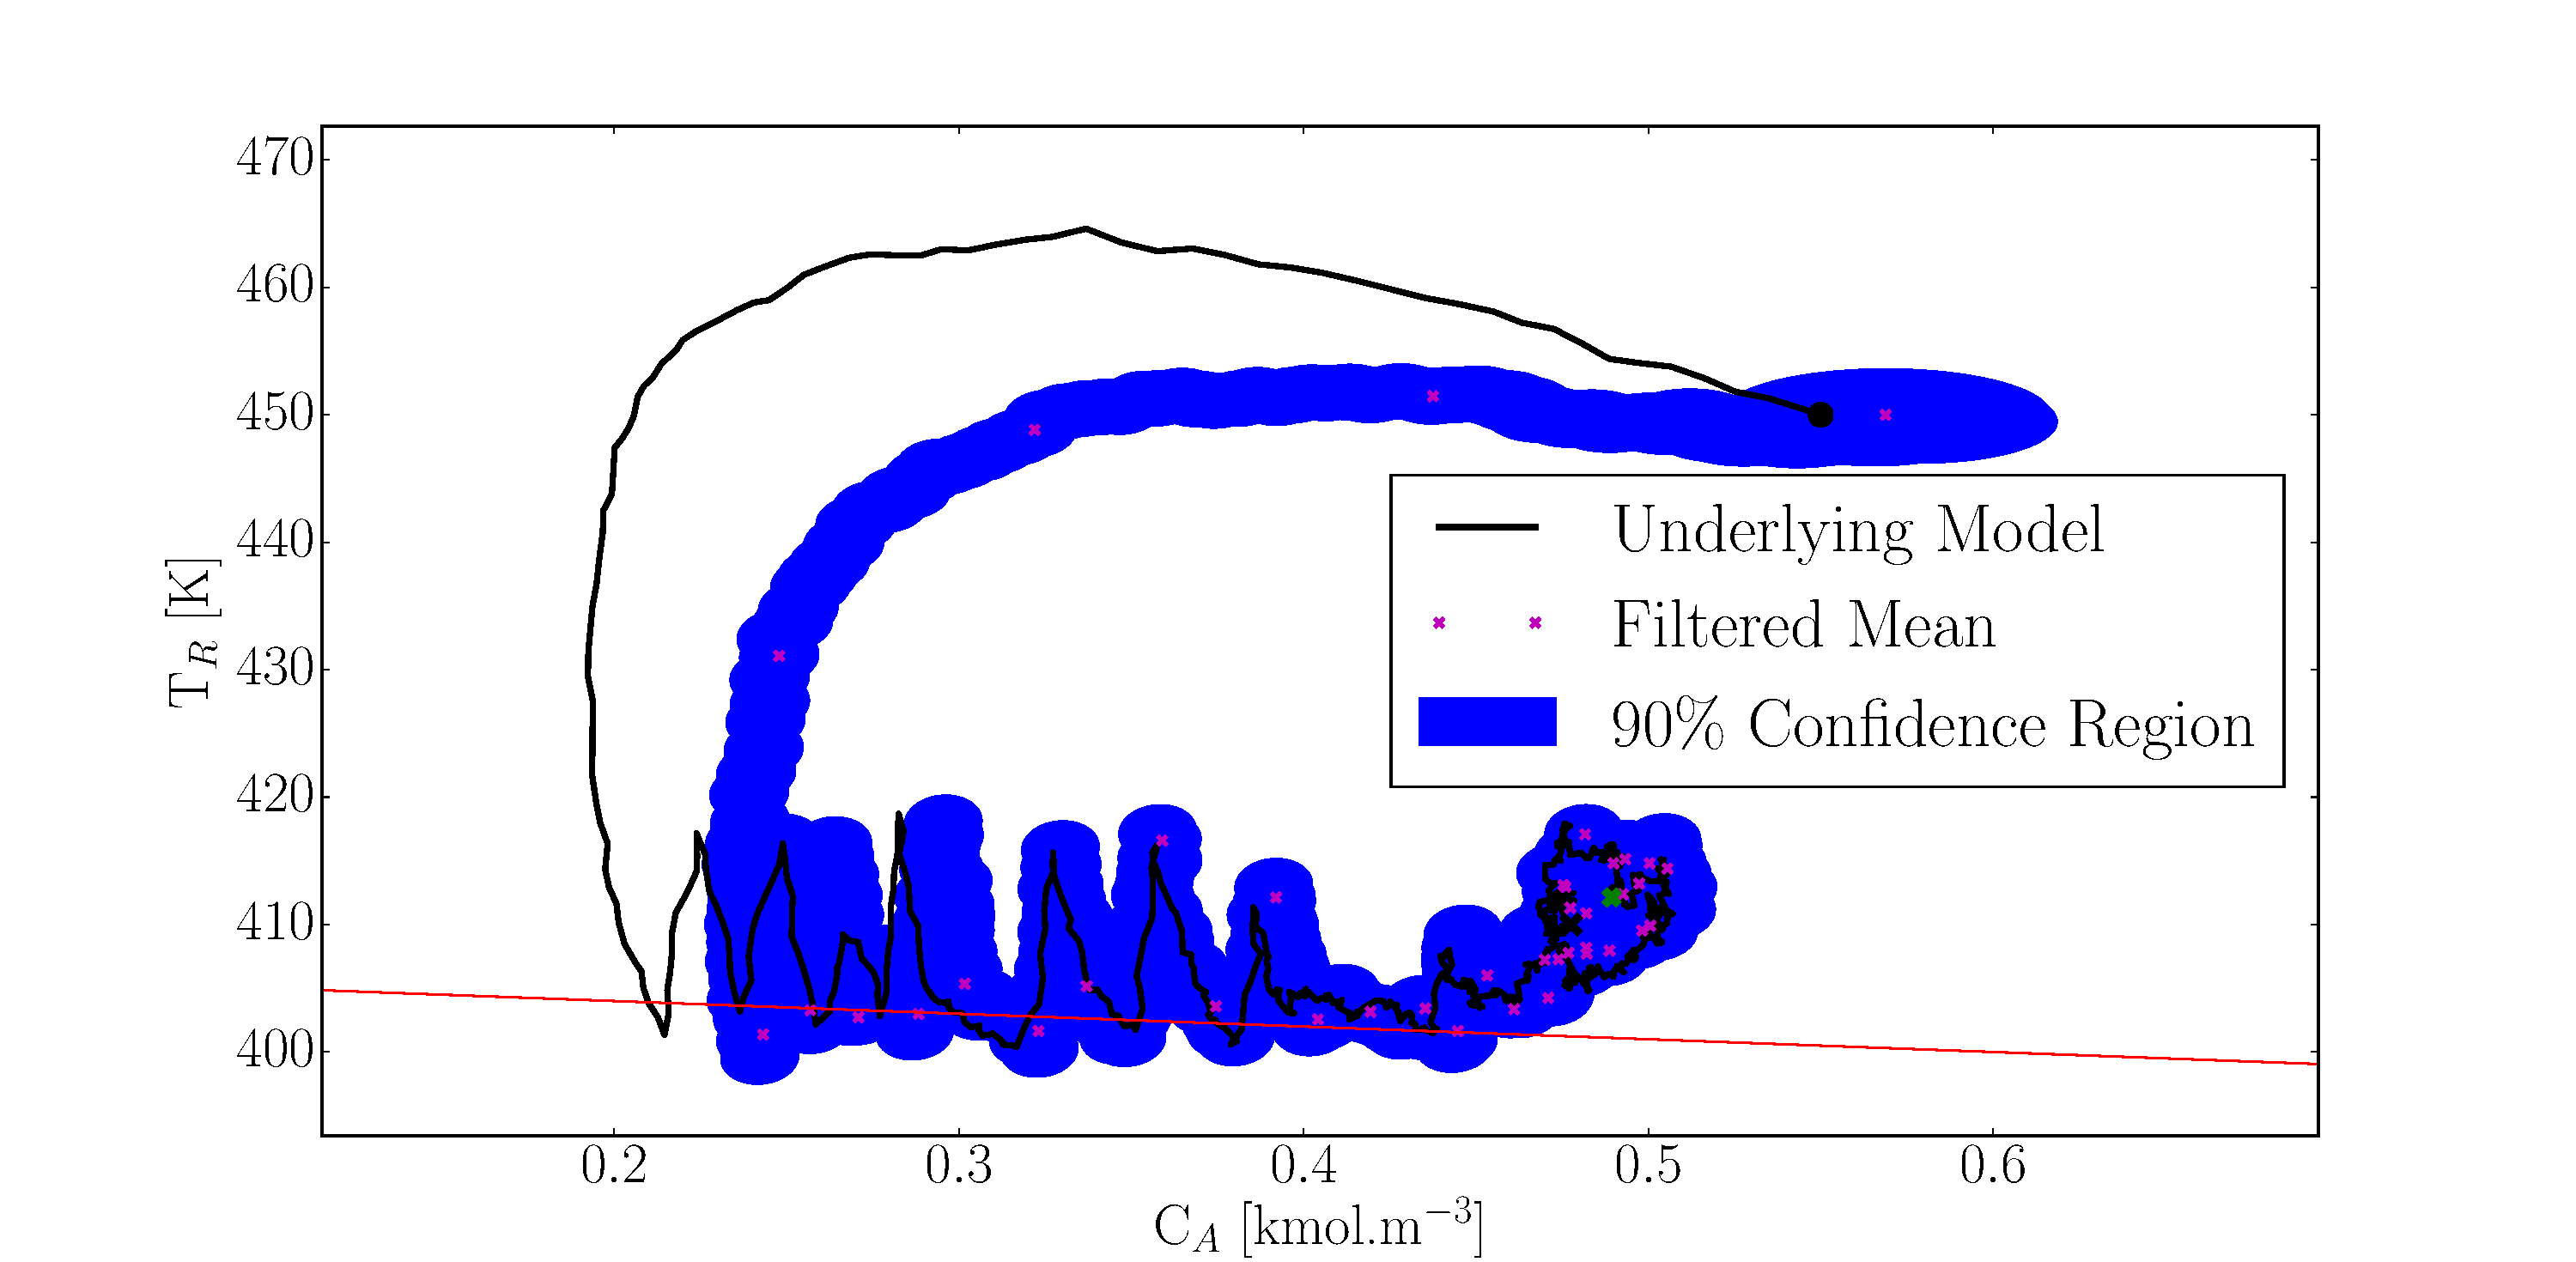
\includegraphics[scale=0.25]{nonlin_mod_kf_mean_ss.pdf}
\caption{Deterministic constrained MPC state space trajectory with initial condition $(0.55, 450)$ and measuring both states. The Kalman Filter is used for inference.}
\label{fig_nonlin_mod_kf_mean_ss}
\end{figure}
Since we are not using a stochastic MPC the state constraint violation is not surprising in Figure \ref{fig_nonlin_mod_kf_mean_ss}. However, a more significant issue is the inability of the Kalman Filter to accurately track the states throughout the simulation (the underlying system briefly diverges from the state estimates). This can be significantly problematic if a constraint existed in the left hand side of the state space: the controller wouldn't know that it was violating the constraint because the state estimate is poor. This behaviour is caused by the linear model used by the Kalman Filter. The state trajectory moves away from the region close to the linearisation point and thus, as explained in Section \ref{sec_inf_lin_mods}, the state estimate becomes poor.

We can remedy this situation by using a more sophisticated inference algorithm. In Figure \ref{fig_nonlin_mod_pf_mean_track} we see the deterministic MPC using a Particle Filter with 200 particles for inference. 
\begin{figure}[H] 
\centering
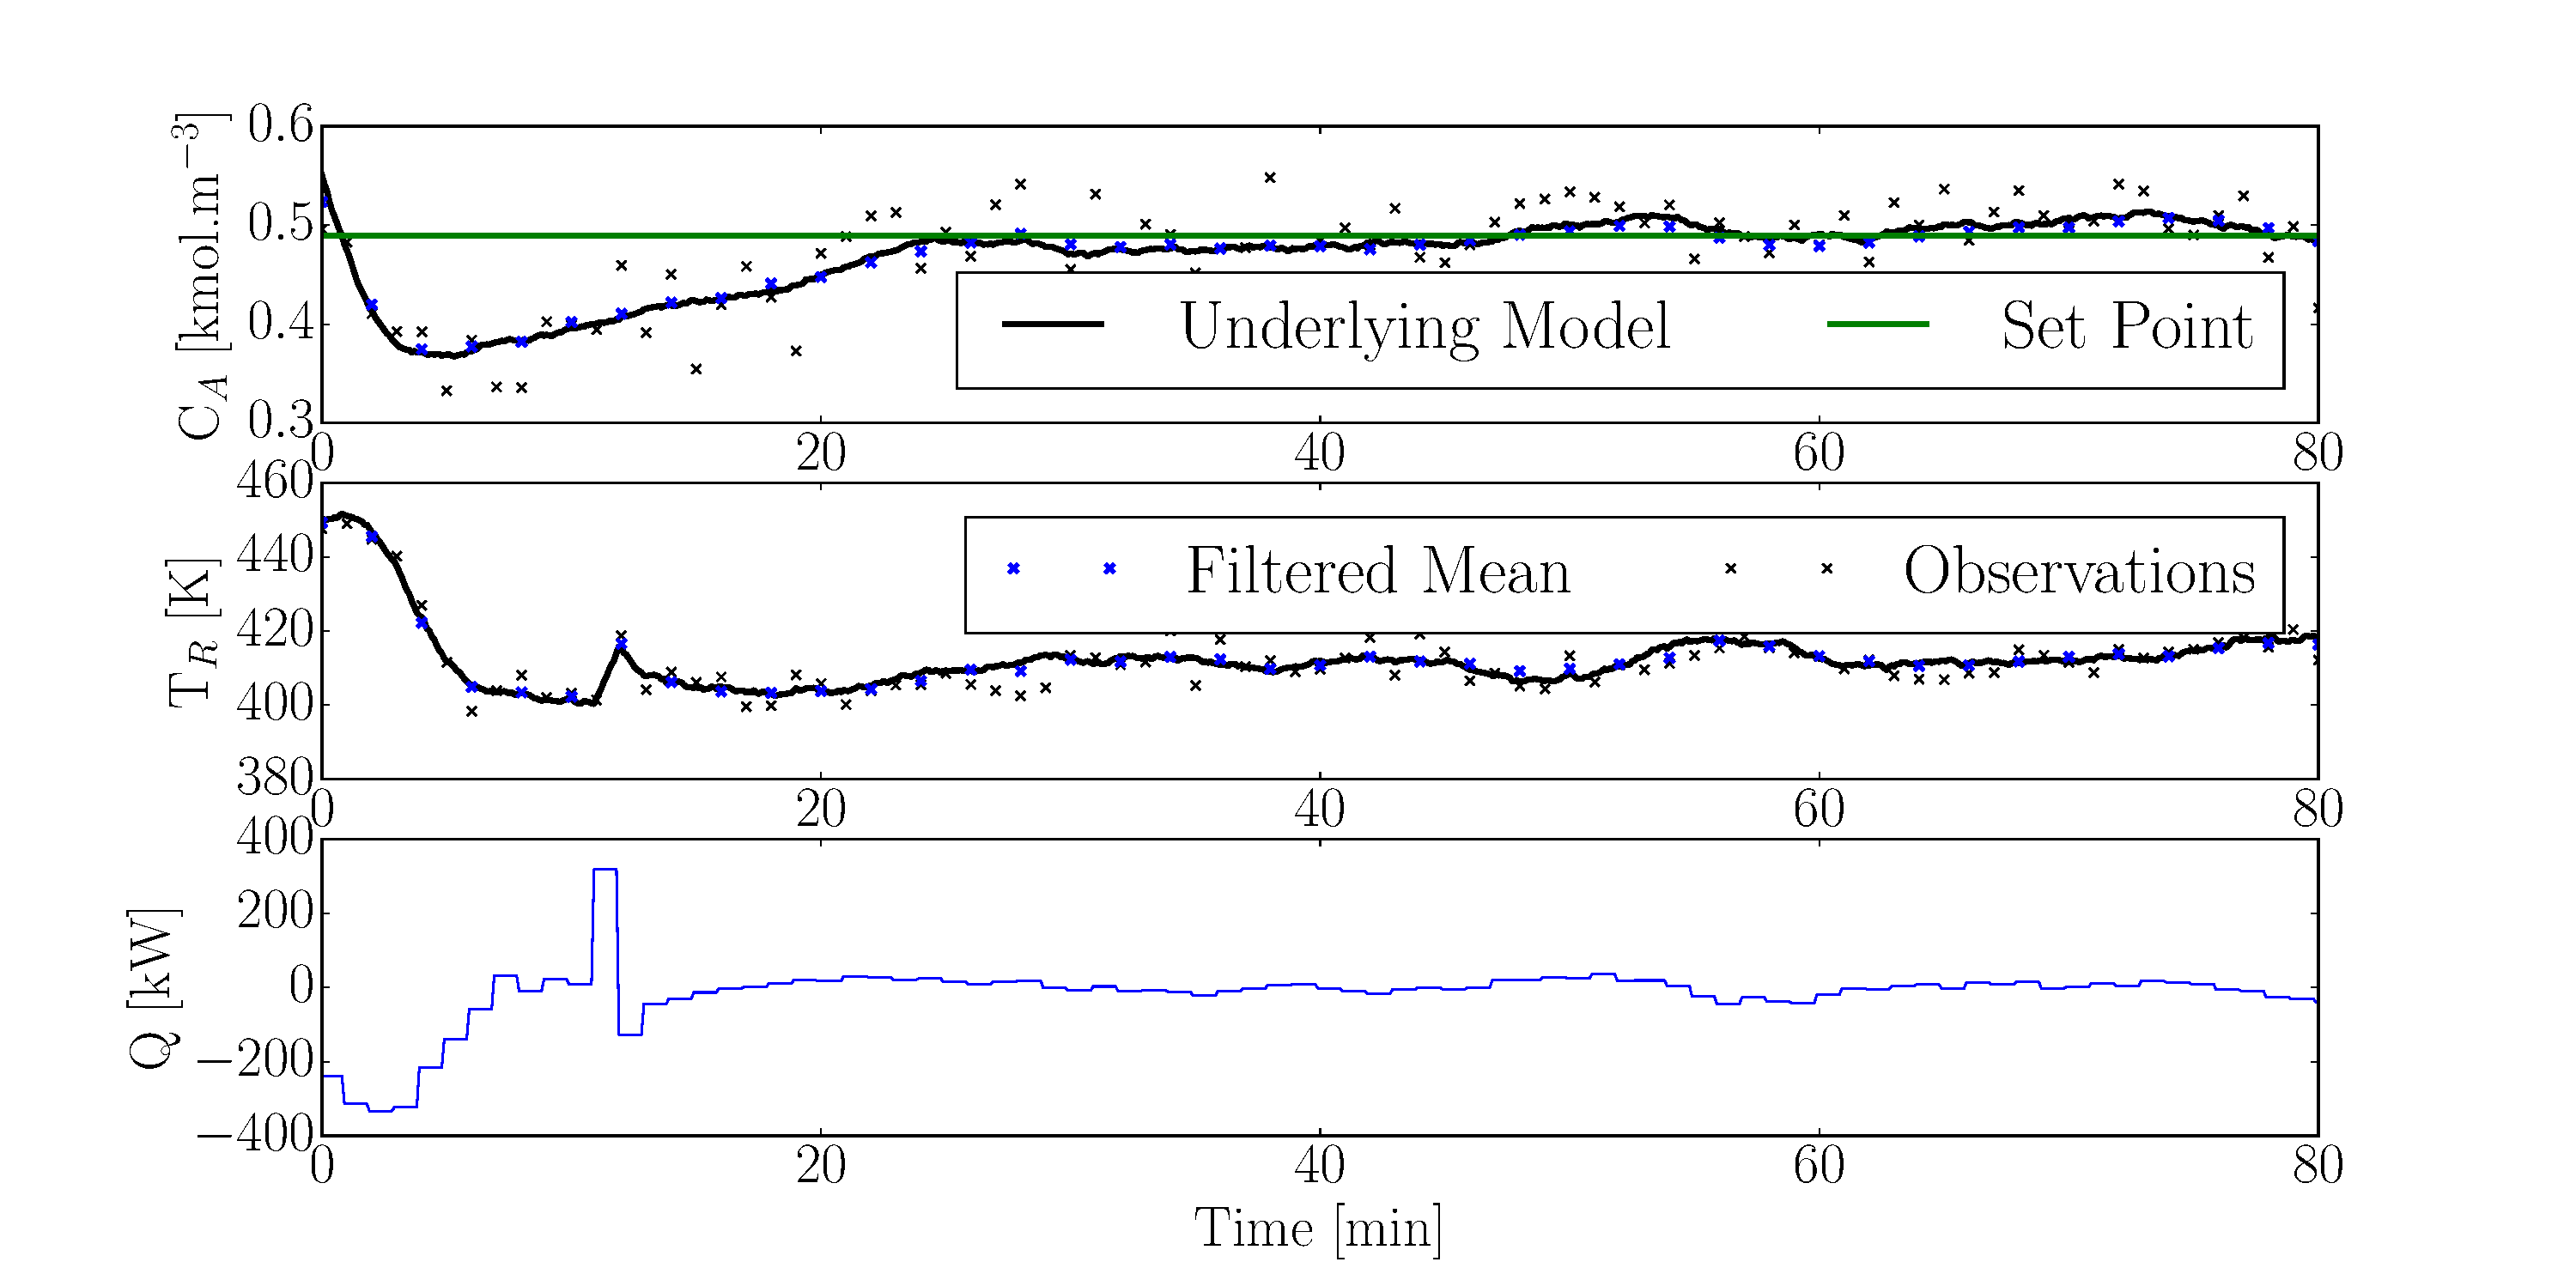
\includegraphics[scale=0.25]{nonlin_mod_pf_mean_track.pdf}
\caption{Deterministic constrained MPC reference tracking with initial condition $(0.55, 450)$ and measuring both states. A Particle Filter with 200 particles is used for inference.}
\label{fig_nonlin_mod_pf_mean_track}
\end{figure} 
The average energy input and concentration error is 218 kJ/min and 4.80\% respectively. This is a vast improvement over the same controller where the Kalman Filter was used for inference. The benefit of accurate state estimation is apparent here and also in Figure \ref{fig_nonlin_mod_pf_mean_ss}.
\begin{figure}[H] 
\centering
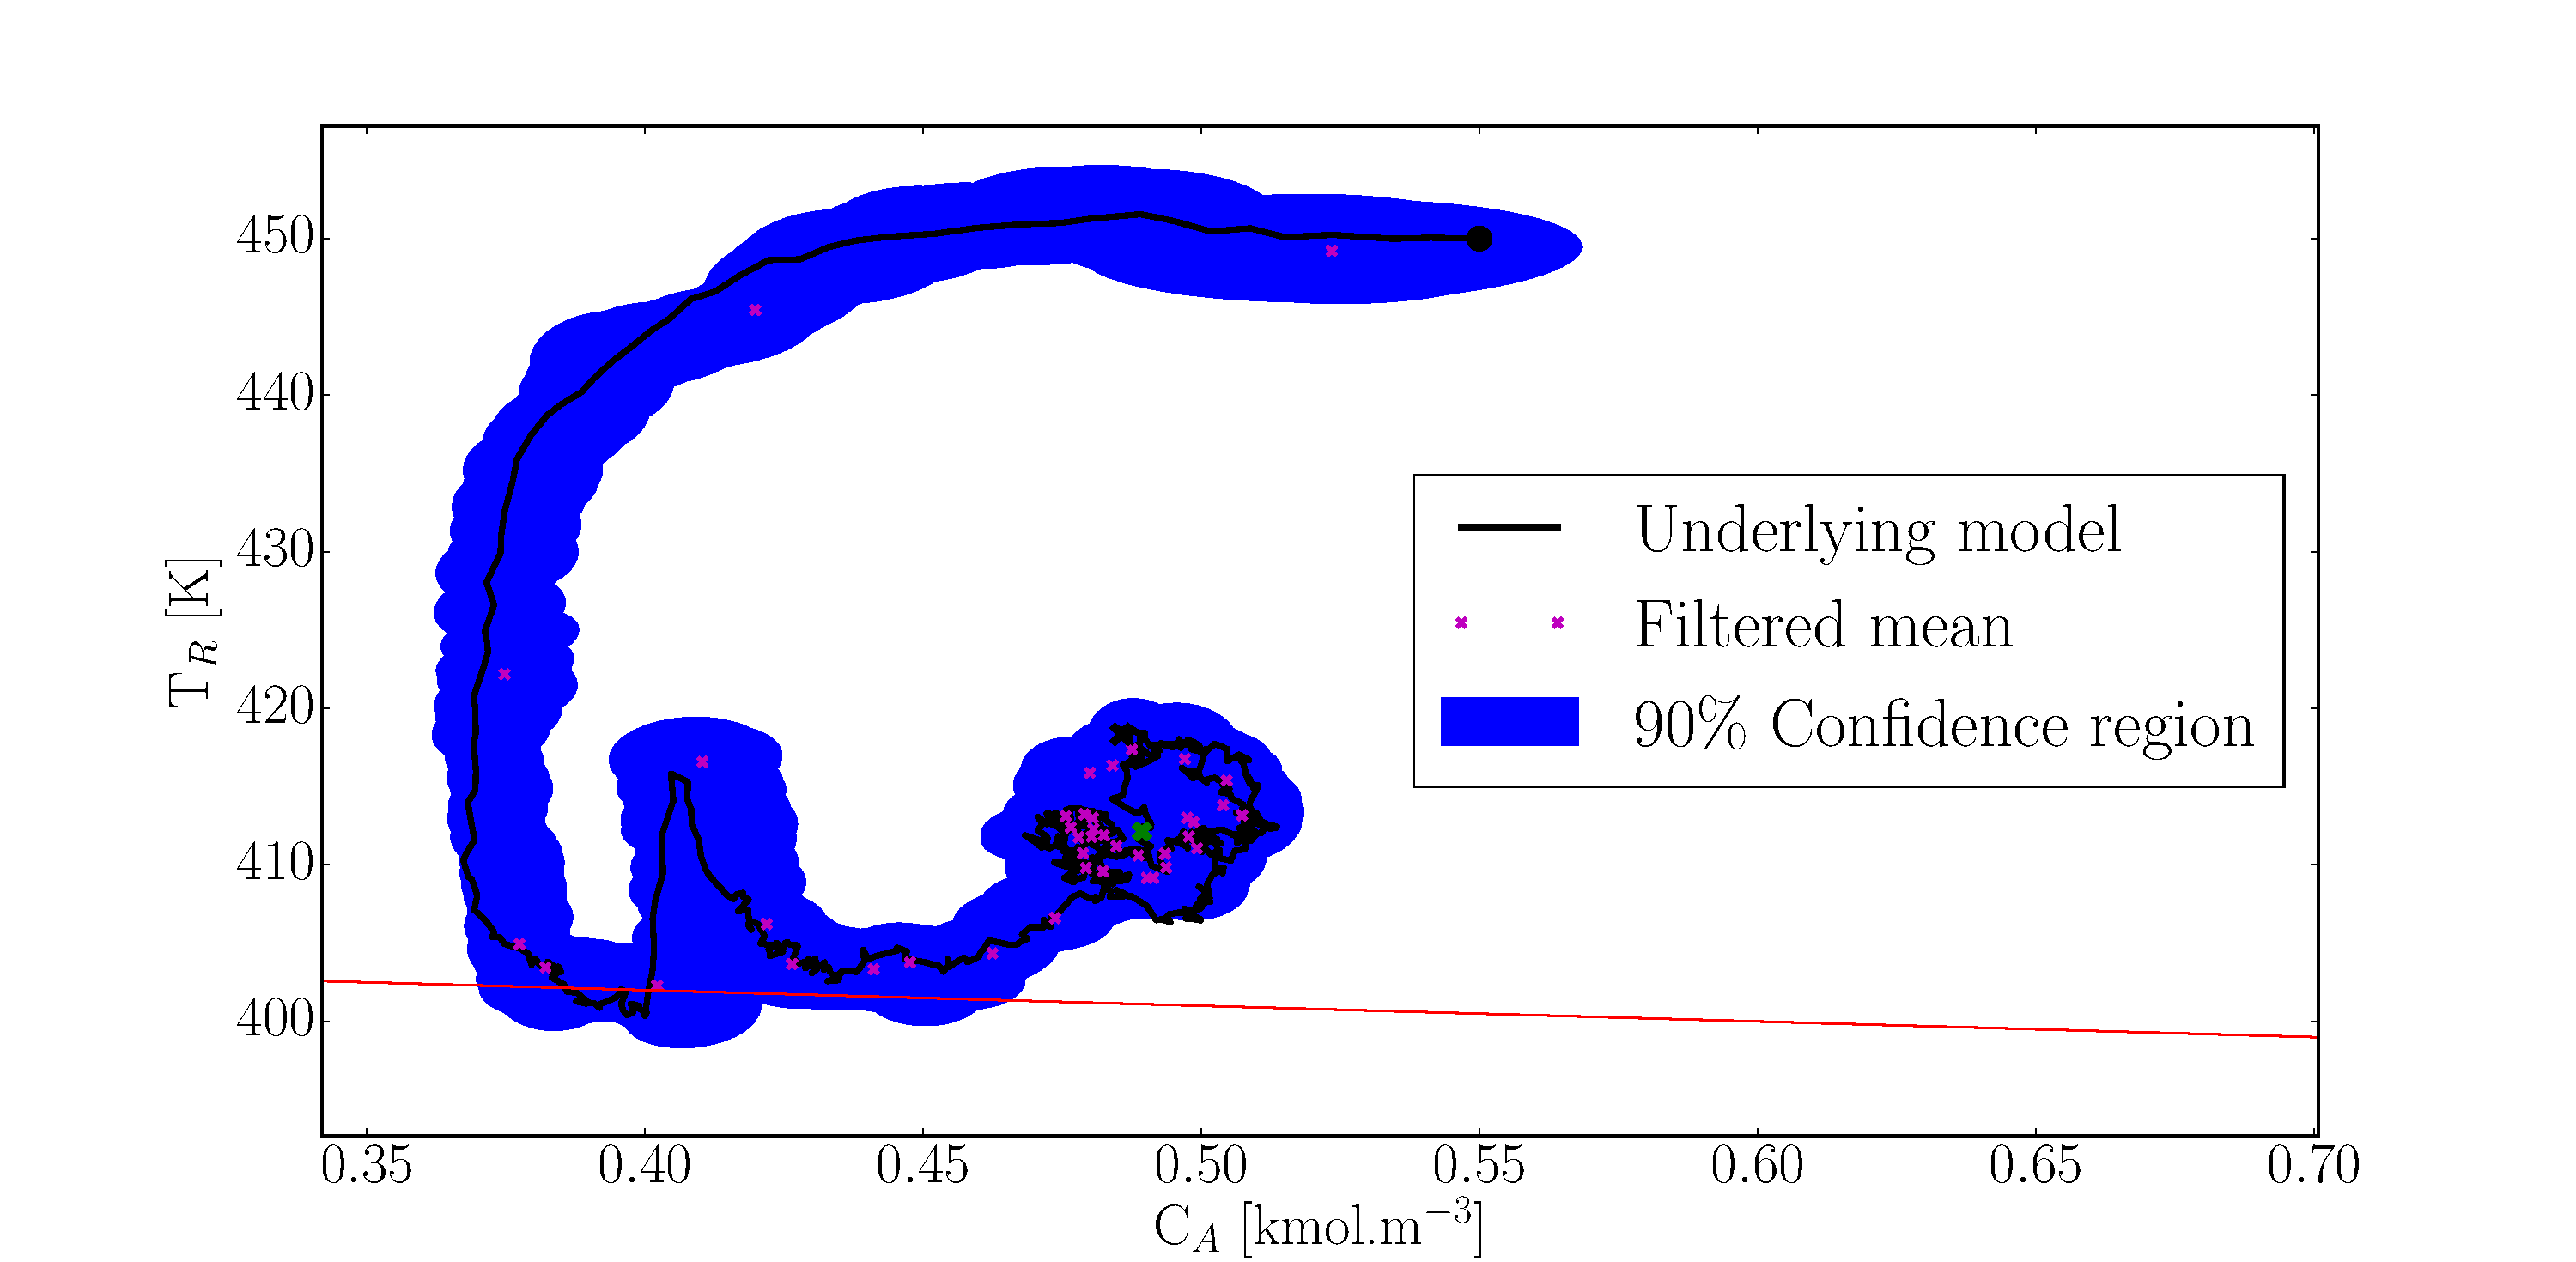
\includegraphics[scale=0.25]{nonlin_mod_pf_mean_ss.pdf}
\caption{Deterministic constrained MPC state space trajectory with initial condition $(0.55, 450)$ and measuring both states. A Particle Filter with 200 particles is used for inference.}
\label{fig_nonlin_mod_pf_mean_ss}
\end{figure}
In Figure \ref{fig_nonlin_mod_kf_mean_ss} we saw significant estimation deviation from the true underlying model, while in Figure \ref{fig_nonlin_mod_pf_mean_ss} the deviation is negligible. We still have that the state constraint is violated but this is due to the stochastic nature of the underlying system.

 